\documentclass[a4paper]{cas-dc}

\usepackage[T1]{fontenc}
\usepackage[utf8]{inputenc}

\usepackage{microtype}

\emergencystretch=2em

\usepackage[english]{babel}
\usepackage{csquotes}

\usepackage{amsmath}
\usepackage{amssymb}
\usepackage{amsthm}

\usepackage{booktabs}
\usepackage{multirow}
\usepackage{graphicx}
\usepackage{multicol}
\graphicspath{{./}}

\usepackage{flushend}

\setlength{\intextsep}{6pt plus 2pt minus 2pt}
\setlength{\textfloatsep}{8pt plus 2pt minus 2pt}
\setlength{\floatsep}{6pt plus 2pt minus 2pt}
\setlength{\abovecaptionskip}{4pt}
\setlength{\belowcaptionskip}{2pt}

\renewcommand{\topfraction}{0.92}
\renewcommand{\bottomfraction}{0.6}
\renewcommand{\textfraction}{0.06}
\renewcommand{\floatpagefraction}{0.55}
\renewcommand{\dbltopfraction}{0.92}
\renewcommand{\dblfloatpagefraction}{0.55}
\setcounter{topnumber}{4}
\setcounter{bottomnumber}{3}
\setcounter{totalnumber}{6}
\setcounter{dbltopnumber}{3}

\usepackage{enumitem}
\setlist{noitemsep, topsep=3pt, partopsep=0pt}

\usepackage[backend=biber,style=apa,sorting=nyt,maxbibnames=99]{biblatex}
\addbibresource{references.bib}
\renewcommand*{\bibfont}{\small}
\setlength{\bibitemsep}{0pt}
\setlength{\bibhang}{1em}

\usepackage{lastpage}
\usepackage{orcidlink}
\hypersetup{colorlinks=true, linkcolor=blue, citecolor=blue, urlcolor=blue}
\usepackage[capitalise]{cleveref}

\usepackage[version=4]{mhchem}

\newcommand{\fechapreprint}{6 October 2026}

\ExplSyntaxOn
\cs_set:Npn \__first_footerline:
  { \group_begin: \small \sffamily \__short_authors: :~
     { \rmfamily \itshape Preprint,~\fechapreprint } \group_end: }
\cs_set:Npn \__cas_foot:
  { \parbox[t]{\textwidth}
     { \rule{\textwidth}{.2pt}\\ \sffamily\small \__first_footerline:
        \hfill Page~\thepage{}~of~\pageref*{LastPage} } }
\cs_set_eq:NN \__first_foot: \__cas_foot:
\RenewDocumentEnvironment { keywords } { O{ Keywords } }
  { \tex_global:D \tex_setbox:D \g_stm_key_box = \vtop \bgroup
     \hsize=.25 \textwidth
     \cs_set_eq:NN \sep \par
     \parindent \c_zero_dim
     A\,R\,T\,I\,C\,L\,E\ \ I\,N\,F\,O \par \skip_vertical:n { -3pt }
     \rule{.25 \textwidth}{.2pt}\par\footnotesize
     \noindent \textit { #1 }:  \par }
  { \egroup }
\RenewDocumentCommand \printorcid { }
  { \seq_if_empty:NF \g_stm_orcid_seq
      { \group_begin: \tex_let:D \thefootnote \relax \footnotetext
          { \raggedright \textsc{orcid}(s):\c_space_token
            \seq_use:Nn \g_stm_orcid_seq { ;~ } }
        \group_end: } }
\ExplSyntaxOff
\addto\captionsenglish{\renewcommand\abstractname{A\,B\,S\,T\,R\,A\,C\,T}}
\pagestyle{cas}

\shorttitle{Daily ozone exceedances in the Monterrey Metropolitan Area}
\shortauthors{A. Eduardo-Luna et al.}

\begin{document}

\title[mode=title]{Discriminating daily ozone exceedances in the Monterrey Metropolitan Area}
\title[mode=sub]{Station-day classification under the 51 ppb threshold of NOM-020-SSA1-2021 at 15 SIMA stations, 2021--2025}

\author[1]{Angel Eduardo-Luna\texorpdfstring{\,\orcidlink{0009-0004-8217-9688}}{}}
\author[1]{Jenaro Alcaraz}
\author[1]{Emilia Rico}
\author[1]{Mar Fernández}
\author[1]{Sofía Fernández}

\affiliation[1]{organization={Instituto Tecnológico y de Estudios Superiores de Monterrey},
  city={Monterrey}, state={Nuevo León}, country={Mexico}}

\begin{abstract}
This work discriminates ozone exceedance days in the Monterrey Metropolitan
Area, defined as a daily maximum 8-hour average (MDA8) above 51 ppb, the
5-year target of the Mexican standard NOM-020-SSA1-2021. Hourly records from
15 stations of the Nuevo León Integrated Environmental Monitoring System
(SIMA) between 2021 and 2025 are aggregated into 25,100 station-days; the
years 2021--2024 are used for fitting and 2025 for validation. An exploratory
factor analysis reduces 13 meteorological and primary-pollutant predictors to
three factors ---primary combustion, ventilation and photochemical
forcing--- that are recovered in 2025. On these factors, a logistic regression
and a linear discriminant analysis reach an area under the ROC curve of 0.850
and 0.846 in validation; one additional standard deviation of photochemical
forcing multiplies the odds of exceedance by 2.78, and ventilation is the
only protective factor. An autoregressive logistic model on the metropolitan
series raises the area to 0.898. Exceedance emerges as a seasonal, regional
phenomenon modulated by wind; a year effect that no predictor explains and
the lack of volatile organic compound measurements are the main limitations.
\end{abstract}

\begin{keywords}
tropospheric ozone \sep factor analysis \sep principal component analysis
\sep logistic regression \sep linear discriminant analysis \sep
autoregressive model \sep Monterrey Metropolitan Area
\end{keywords}

\maketitle
\hypersetup{pdftitle={Discriminating daily ozone exceedances in the Monterrey Metropolitan Area},
  pdfauthor={Angel Eduardo-Luna, Jenaro Alcaraz, Emilia Rico, Mar Fernández, Sofía Fernández},
  pdfsubject={}, pdfkeywords={tropospheric ozone; factor analysis; principal component analysis; logistic regression; linear discriminant analysis; autoregressive model; Monterrey Metropolitan Area}}

\section{Introduction and rationale}
\label{sec:introduccion}

Air quality in Nuevo León is a key determinant of public health: daily
exposure to high pollutant concentrations poses a cumulative risk to the
population. The continuous measurements of the Integrated Environmental
Monitoring System (SIMA), described in \cref{sec:sima}, make it possible to
characterize the atmosphere of the Monterrey Metropolitan Area (MMA) and are
the data source of this work. To report air quality, SIMA converts hourly
measurements into a categorical index with a color associated with its
maximum value \parencite{aireNL2026}.

Of the pollutants measured by the network, tropospheric ozone is the one
that motivates this study: it is a secondary pollutant, formed rather than
emitted, and its formation depends jointly on chemical precursors and on
meteorological conditions. That dual dependence is what makes a
multivariate analysis appropriate: no single variable explains an
exceedance day.

\subsection{Tropospheric ozone}
\label{sec:objetivo}

Ozone (\ce{O3}) is a molecule of three oxygen atoms found both in the upper
atmosphere (stratospheric ozone) and at ground level (tropospheric ozone).
Stratospheric ozone is produced naturally by the interaction of molecular
oxygen (\ce{O2}) with ultraviolet radiation, and it attenuates the exposure
of the surface to that radiation \parencite{Bernhard2023-lk}. Tropospheric
ozone, by contrast, is the main ingredient of \textit{smog} and forms through
chemical reactions between nitrogen oxides (\ce{NOx}) and volatile organic
compounds (VOCs) in the presence of heat and sunlight.

Highly industrialized metropolitan areas of Nuevo León have recorded
\ce{O3} and \ce{PM10} levels above the limits of the Mexican standards
NOM-020-SSA1-2021 \parencite{nom020ssa1} and NOM-025-SSA1-2021
\parencite{nom025ssa1}. These trends have been documented for more than
30 years with instruments that measure both ozone (ultraviolet photometry)
and its precursors \ce{NO} and \ce{NO2} (grouped as \ce{NO_x}, by
chemiluminescence), whose photochemical relationship is key to understanding
the formation of the secondary pollutant \parencite{SanfordSillman}.

The MMA is no exception: between 1993 and 2014 tropospheric ozone
concentrations rose steadily, in contrast with the declining trend in Mexico
City over the same period. The increase has been attributed to industrial and
vehicular growth without equivalent control of precursors, and to a
meteorological role modulated by climate change \parencite{atmos15070779}.
The topography of the valley in which the MMA lies aggravates this behavior:
the surrounding mountain ranges favor the stagnation of air masses during
episodes of high pressure, thermal inversion and weak wind, which reduce
dispersion and prolong the exposure of the population.

\subsection{Environment and health}
\label{sec:revi-medio-ambiente}

Air pollution is a health risk associated with conditions such as heart
disease, stroke, pneumonia, lung cancer and respiratory infections, mainly
through exposure to particulate matter (\ce{PM2.5} and \ce{PM10}), nitrogen
dioxide (\ce{NO2}), ozone (\ce{O3}) and sulfur dioxide (\ce{SO2}). Air
quality is measured by monitoring stations that record hourly
concentrations, from which metrics such as 24-hour or annual averages are
computed depending on the pollutant, and compared against Mexican official
standards (NOMs) and the recommendations of the World Health Organization
(WHO) \parencite{oms2021}.

Some Mexican limits are less stringent than those recommended by the WHO:
for \ce{PM2.5}, the Mexican annual limit is
$10\,\mu\mathrm{g}/\mathrm{m}^{3}$, whereas the WHO recommends
$5\,\mu\mathrm{g}/\mathrm{m}^{3}$ \parencite{oms2021}. Measurement is further
complicated because not every station measures every pollutant or has
enough valid data, so sufficiency criteria are required, such as having at
least 75\,\% valid data.

The Mexican official standards set concentration limits by pollutant and
exposure period (1 hour, 8 hours, 24 hours or annual average)
\parencite{nlAirenlgobmxNormatividad, NOMCalidadAireAmbiente}. The current
limit values for ozone and particulate matter, which are used as the
exceedance criterion in this work, are given in \cref{tab:nom-limites}.

\subsection{Integrated Environmental Monitoring System (SIMA)}
\label{sec:sima}

The Integrated Environmental Monitoring System (SIMA) is the network of the
Government of Nuevo León responsible for measuring and monitoring air
quality. Its purpose is to determine the pollutant concentrations to which
the population is exposed, to issue alerts when pollution is high, and to
keep citizens informed about environmental health and air quality
\parencite{gobiernoNL2026PIGECA}.

SIMA began operating on 20 November 1992 as a department of the
Undersecretariat for Environmental Protection and Natural Resources, with
five monitoring stations. Over 32 years it has expanded and modernized its
infrastructure \parencite{villasaez2024}. It currently operates 15 fixed
stations distributed across 11 municipalities of the Monterrey metropolitan
area, plus 2 mobile stations \parencite{gobiernoNL2026ModernizacionSIMA}.

SIMA measures eight criteria pollutants and seven meteorological parameters,
listed with their units and coverage in the data dictionary
(\cref{tab:dic-contaminantes,tab:dic-meteo}).

SIMA is the government infrastructure that turns information on air
pollution into environmental management actions, and it is the direct
source of the data used in this work.

\subsection{The stations and their geographic context}
\label{sec:contexto-estaciones}

The MMA occupies a valley at about 500 m above sea level (a.s.l.), bounded to
the south and west by the Sierra Madre Oriental, to the east by Cerro de la
Silla and to the north by Cerro del Topo Chico and Sierra de las Mitras. The
15 SIMA stations are spread across this valley along an elevation gradient
from 334 m a.s.l., on the southeastern plain, to 702 m a.s.l., at the foot of
the mountains in the northwest (\cref{tab:estaciones}). Each station code
indicates its quadrant, and from it the stations are grouped into seven
zones that the models of \cref{sec:clasificacion_tecs} use as a categorical
predictor.

\begin{table}[pos=t]
  \centering
  \caption{SIMA stations, the zone to which each is assigned, and elevation.
    Coordinates in degrees and minutes; all north latitude and west
    longitude.}
  \label{tab:estaciones}
  \small
  \begin{tabular}{llrll}
    \toprule
    Code & Zone & m a.s.l. & Lat. & Long. \\
    \midrule
    \texttt{SE3}  & Southeast & 334 & 25°36' & 100°00'  \\
    \texttt{NE3}  & Northeast & 346 & 25°47' & 100°05' \\
    \texttt{SE2}  & Southeast & 387 & 25°39' & 100°06' \\
    \texttt{NE2}  & Northeast & 432 & 25°47' & 100°11' \\
    \texttt{NE}   & Northeast & 474 & 25°45' & 100°15' \\
    \texttt{SE}   & Southeast & 500 & 25°40' & 100°15' \\
    \texttt{NTE}  & North     & 503 & 25°48' & 100°20' \\
    \texttt{NTE2} & North     & 520 & 25°44' & 100°19' \\
    \texttt{SUR}  & South     & 555 & 25°37' & 100°16' \\
    \texttt{CE}   & Center    & 562 & 25°41' & 100°20' \\
    \texttt{NO}   & Northwest & 568 & 25°46' & 100°22' \\
    \texttt{NO3}  & Northwest & 607 & 25°46' & 100°28' \\
    \texttt{SO2}  & Southwest & 636 & 25°40' & 100°25' \\
    \texttt{SO}   & Southwest & 674 & 25°41' & 100°27' \\
    \texttt{NO2}  & Northwest & 702 & 25°48' & 100°35' \\
    \bottomrule
  \end{tabular}
\end{table}

Three geographic factors shape the measurements. The first is wind: the
median zonal wind component is negative (\cref{tab:cuartiles-iqr}), that is,
the prevailing wind enters from the east and carries the precursors emitted
in the center and east of the city toward the west, where the mountains
block their exit. The second is elevation, which covaries with distance to
\ce{NOx} sources and with land use: the correlation between a station's
elevation and its exceedance rate is 0.827 across the 15 stations
(\cref{fig:elevacion-excedencia}). The third is the orographic enclosure
already described in \cref{sec:objetivo}, which prevents vertical and
horizontal dispersion during episodes of high pressure and weak wind. The
result is a west--east ordering that is stable across the four seasons: the
Northwest and Southwest have the highest exceedance rates (43.3\,\% and
42.1\,\%) and the Northeast the lowest (19.5\,\%).

\begin{figure}[pos=t]
  \centering
  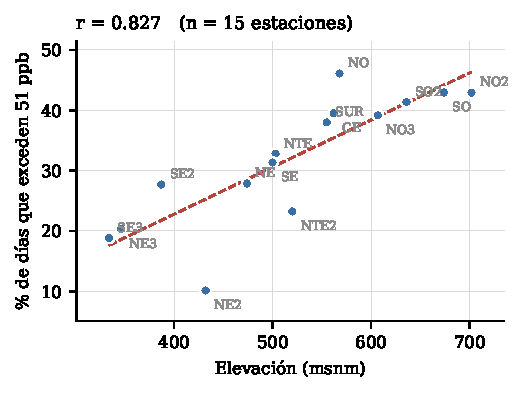
\includegraphics[width=\linewidth]{elevacion_vs_excedencia.pdf}
  \caption{MDA8 exceedance rate at 51 ppb versus the elevation of each
    station, 2021--2025. With $n=15$ and correlated neighboring stations,
    the line describes an association, not an effect of altitude.}
  \label{fig:elevacion-excedencia}
\end{figure}

Two considerations limit comparability across stations. \texttt{NO3} has
operated only since December 2022, so its window is shorter; and no station
measures volatile organic compounds, the second ozone precursor, which
restricts any chemical interpretation to nitrogen oxides, with \ce{CO} as a proxy.


\section{Problem and objective}
\label{sec:objetivo-tecnicas}

\subsection{Problem}

The MMA has accumulated three decades of rising ozone (\cref{sec:objetivo}),
and its monitoring network produces, every hour and at 15 sites, the
concentrations of the precursors and the meteorological conditions that
govern its formation. The question this work addresses is which combination
of those conditions accompanies a day on which ozone exceeds the standard,
and how reliably such a day can be identified from them. Two obstacles make
it a multivariate problem rather than a comparison of thresholds: the
precursors are strongly correlated with one another (\ce{NO}, \ce{NO2} and
\ce{NOx} are the same emission measured three times), and the response is
rare under the current threshold, so a trivial rule is almost always right
without saying anything.

\subsection{Objective of the multivariate analysis}
\label{sec:obj:objetivo}

\textbf{Main objective.} To classify each station-day record as an
exceedance or non-exceedance of the MDA8 at the 51 ppb threshold, from the
same-day precursors and meteorological variables, and to identify which
latent conditions explain that classification.

\textit{Performance criterion:} area under the ROC curve $\geq 0.75$ on a
validation partition not seen during fitting, with sensitivity and
specificity reported separately. Accuracy is not used: under the current
65 ppb threshold, exceedances are 11.25\,\% of valid station-days, and a
constant classifier would reach 88.75\,\% accuracy without identifying the
phenomenon (\cref{sec:eda-cualitativas}). For that reason the main scenario
uses 51 ppb, the 5-year target of NOM-020-SSA1-2021 (\cref{tab:nom-limites}),
with 31.96\,\% exceedances \parencite{saito2015}.

Stations are not grouped by their mean ozone levels, which the station
explains in only 5.3\,\% of the MDA8 variance; instead they are assigned to
the seven zones of \cref{sec:contexto-estaciones}, whose spatial content is
supported by the data.

\subsection{Statistical techniques}
\label{sec:obj:tecnicas}

Interdependence techniques, which reduce the predictors to interpretable
axes, are combined with dependence techniques, which relate those axes to
exceedance:

\begin{itemize}
  \item \textbf{Principal component analysis (PCA)}: resolves the
    multicollinearity of the predictors and yields orthogonal axes with a
    physical interpretation.
  \item \textbf{Exploratory factor analysis (FA)}: separates common from
    specific variance and exposes redundancies that PCA absorbs without
    flagging. Its scores are the predictors of the classification models.
  \item \textbf{Logistic regression}: models the probability of exceedance
    and the contribution of each predictor as an odds ratio, without
    normality assumptions; it has already been applied to MDA8 exceedance
    from meteorological variables \parencite{otero2016}.
  \item \textbf{Linear discriminant analysis}: contrasts the logistic model
    under the assumptions of multivariate normality and equal covariances
    \parencite{hosmer2013}. Box-Cox left the skewness at
    $|\text{skewness}|<0.5$ (\cref{tab:sesgos-transformacion}), which
    approximates the first assumption.
  \item \textbf{Autoregressive logistic model}: incorporates the temporal
    dependence of the response, which the time-series characterization shows
    to persist after removing seasonality.
\end{itemize}

All classifiers are evaluated with the area under the ROC curve, not with
accuracy, because of the imbalance noted above \parencite{saito2015}. The
standardization of \cref{sec:transformaciones} is required: in original
units, pressure, with values near 710, would dominate distances over
\ce{CO}, whose values are below 10.

\subsection{Variables and their characteristics}
\label{sec:obj:variables}

Definitions, units and missing data are given in the data dictionary
(\cref{sec:diccionario}); \cref{tab:variables-tecnica} presents the role of
each group of variables in the objective.

\begin{table}[pos=t]
  \centering
  \caption{Role of each group of variables in the objective.}
  \label{tab:variables-tecnica}
  \footnotesize
  \begin{tabular}{@{}p{3.2cm} p{4.4cm}@{}}
    \toprule
    Group & Role \\
    \midrule
    \ce{O3}, MDA8 & Define the class; not predictors \\
    \addlinespace[2pt]
    \ce{NO}, \ce{NO2}, \ce{NO_x}, \ce{CO} & Predictors, morning window
      06--09 h \parencite{abdulwahab2005} \\
    \addlinespace[2pt]
    \ce{PM10}, \ce{PM_{2.5}}, \ce{SO2} & Predictors, daily mean \\
    \addlinespace[2pt]
    \texttt{TOUT}, \texttt{RH}, \texttt{SR}, \texttt{PRS}, \texttt{WSR},
      \texttt{viento\_u}, \texttt{viento\_v} & Predictors, daily summaries
      (maximum, total, mean, minimum) \\
    \addlinespace[2pt]
    \texttt{temporada}, \texttt{tipo\_dia}, \texttt{zona} & Categorical
      predictors (season, day type, zone), coded as $k-1$ indicators \\
    \bottomrule
  \end{tabular}
\end{table}

Precursors are summarized over the 06--09 h window because morning emissions
feed midday photochemistry; solar radiation is retained to distinguish
aerosol attenuation from a difference in light availability. Categorical
variables enter as $k-1$ indicators with an explicit reference category
(Northeast, weekday and winter); including all $k$ levels would create
perfect collinearity with the intercept. PCA and FA exclude these indicators
because the binary columns would artificially inflate the explained
variance.


\section{Data preparation}
\label{sec:preparacion-datos}

\subsection{Consolidation and cleaning}

The six annual SIMA files do not share a structure: the headers, the
position of the units row and the number of stations change (13 in 2020,
15 from 2022 onward). They are consolidated into a single hourly table of
15 parameters by station and date, 754,603 records between 2020 and 2025.
The quality audit detects sentinel values ($-9999$, the logger's missing-data
code) and physically impossible values (relative humidity of up to
725\,\%, temperatures of 785\,°C), which are set to missing rather than
imputed; details are given in the data dictionary (\cref{sec:dic:centinela}).
The share of missing data per parameter ranges from 3.66\,\% for solar
radiation to 25.23\,\% for \ce{PM_{2.5}}, but it is not evenly distributed
across years or stations, which determines the study window.

\subsection{Data selection}

The dataset for the subsequent steps is built from the data dictionary and
the quality diagnosis.

Since the objective is to analyze the behavior of tropospheric ozone, each
variable is assessed to determine, based on the literature, whether there is
a documented mechanism ---chemical, physical or meteorological--- through
which it influences \ce{O3} formation.

The target variable is the \ce{O3} from the database:

\begin{table*}[pos=t]
  \centering
  \caption{Target variable: tropospheric ozone (\ce{O3}).}
  \label{tab:variable-objetivo}
  \begin{tabular}{lcccc}
    \toprule
    Unit & Operating range & Observed range & Median & Missing (\%) \\
    \midrule
    ppb & 0--153 to 0--185 & 0.5--265.0 & 23.00 & 14.73 \\
    \bottomrule
  \end{tabular}
\end{table*}

\begin{quote}
    Stations report results every hour, i.e., 24 measurements per day. The
    regulatory MDA8 metric collapses those 24 measurements into a single
    value per station and day, since NOM-020-SSA1 sets the ozone limit on
    the 8-hour average, not on the hourly value.
\end{quote}

\Cref{tab:nom-limites} lists the current Mexican limit values for ozone and
particulate matter. Note that the regulatory indicator for \ce{O3} is not the
hourly concentration but the 8-hour moving average, and that the evaluation
criterion is the maximum of the daily maxima of those averages; this
justifies adopting the daily maximum 8-hour moving average (MDA8) as the
target variable of the analysis.

\begin{table*}[pos=t]
  \centering
  \caption{Current Mexican air quality limit values for the pollutants of
    interest. The years indicate the gradual compliance schedule set by each
    standard \parencite{nom020ssa1, nom025ssa1}.}
  \label{tab:nom-limites}
  \footnotesize
  \begin{tabular}{p{2.6cm} p{7.2cm} ccc}
    \toprule
    & & \multicolumn{3}{c}{Limit value} \\
    \cmidrule(lr){3-5}
    Indicator & Evaluation criterion & Year 1 & Year 3 & Year 5 \\
    \midrule
    \multicolumn{5}{l}{\textbf{\ce{PM10}} ($\mu$g/m$^{3}$) --- NOM-025-SSA1-2021, DOF 27 Oct 2021} \\
    \addlinespace[2pt]
    24 hours & 99th percentile (tolerated frequency: 1\,\% of the time per year) & 70 & 60 & 50 \\
    Annual   & Annual mean of the 24-hour averages                              & 36 & 28 & 20 \\
    \midrule
    \multicolumn{5}{l}{\textbf{\ce{PM_{2.5}}} ($\mu$g/m$^{3}$) --- NOM-025-SSA1-2021, DOF 27 Oct 2021} \\
    \addlinespace[2pt]
    24 hours & 99th percentile (tolerated frequency: 1\,\% of the time per year) & 41 & 33 & 25 \\
    Annual   & Annual mean of the 24-hour averages                              & 10 & 10 & 10 \\
    \midrule
    \multicolumn{5}{l}{\textbf{Ozone} (\ce{O3}, ppm) --- NOM-020-SSA1-2021, DOF 28 Oct 2021} \\
    \addlinespace[2pt]
    1 hour                 & Maximum of the daily maxima of the hourly concentrations                  & 0.090 & 0.090 & 0.090 \\
    8-hour moving average  & Maximum of the daily maxima of the 8-hour moving average concentrations   & 0.065 & 0.060 & 0.051 \\
    \bottomrule
  \end{tabular}
\end{table*}

Missing \ce{O3} values by station and year (\cref{sec:dic:faltantes}) show
that 2020 is unusable: of the 13 stations operating that year, 7 have between
89\,\% and 100\,\% missing data. The year 2020 is discarded entirely.

In 2021 missing data remain high at several stations, but within a range
that allows the analysis; from 2022 onward no station exceeds 20\,\%, except
\texttt{NO3} in 2025 (30.3\,\%). The full years 2021 to 2025 are therefore
retained: 1,826 calendar days.

Within this window, no station has enough missing data to justify excluding
it, so the 15 levels of the variable \texttt{estacion} (station) are kept.
This variable is not subject to the same criterion as the measured
parameters: it is not a physicochemical quantity but an identifier that
defines the spatial structure of the dataset.

Next, the variables that affect tropospheric ozone levels are identified.
Information on the chemical, physical and meteorological processes that
promote or hinder \ce{O3} formation is compiled from the literature.

\begin{itemize}
    \item \textbf{Solar radiation}: in summer, sunlight is more intense and
      temperatures rise, which accelerates photochemical reactions and
      produces higher ozone levels.
    \item \textbf{Quantified seasonal variation}: mean concentrations of
      $45.6\,\mu\mathrm{g}/\mathrm{m}^{3}$ in summer,
      $47.3\,\mu\mathrm{g}/\mathrm{m}^{3}$ in spring,
      $38.0\,\mu\mathrm{g}/\mathrm{m}^{3}$ in autumn and
      $33.6\,\mu\mathrm{g}/\mathrm{m}^{3}$ in winter.
    \item \textbf{Diurnal variation}: ozone levels tend to peak in the late
      afternoon and decrease at night due to the lack of sunlight and to
      titration by \ce{NO}, which consumes ozone.
    \item \textbf{Topography}: valleys surrounded by mountains trap pollutants
      and favor ozone formation (stagnation effect), which applies in
      particular to the Monterrey metropolitan area.
    \item \textbf{Acute events}: heat waves cause atypical short-term
      increases.
\end{itemize}

The chemistry section of Sillman's article \parencite{SanfordSillman}
describes the formation mechanism of tropospheric ozone:

\begin{quote}
    Ozone formation in the lower atmosphere results from a series of
    photochemical reactions involving precursors emitted by natural and
    anthropogenic sources. These reactions begin with the photolysis of
    nitrogen dioxide (\ce{NO2}) under sunlight, which produces atomic oxygen
    (\ce{O}). This atomic oxygen then reacts with molecular oxygen (\ce{O2})
    to form ozone (\ce{O3}).
\end{quote}

The complete cycle:

\begin{enumerate}
    \item $\ce{NO2} + h\nu \to \ce{NO}+\ce{O}$ (photolysis)
    \item $\ce{O} + \ce{O2} + \ce{M} \to \ce{O3} + \ce{M}$ (ozone formation)
    \item VOCs (volatile organic compounds) react with free radicals to
      generate additional \ce{NO2}, feeding the cycle continuously.
\end{enumerate}

From this information, the meteorological variables used in the rest of the
analysis are determined.

\begin{itemize}
    \item \texttt{TOUT} (ambient temperature): the higher the temperature,
      the faster ozone forms.
    \item \texttt{RAINF} (precipitation): precipitation implies cloudy skies,
      which reduce exposure to solar radiation.
    \item \texttt{PRS} (atmospheric pressure): high pressure brings clear,
      cloudless days and near-calm winds, and also acts as a \textit{lid}:
      the heavy air sinks, compresses pollutants against the ground and
      prevents their dispersion.
    \item \texttt{WSR} and \texttt{WDR} (wind speed and direction):
      determine the ability of the atmosphere to disperse pollutants.
\end{itemize}

Among the air pollutants:

\begin{itemize}
    \item \ce{CO} (carbon monoxide) acts as a proxy for the VOCs that react
      with free radicals.
    \item \ce{NO2} is the main ingredient of the photochemical reaction with
      solar radiation.
    \item \ce{NOx} is the group $\ce{NO2} + \ce{NO}$, essential to \ce{O3}
      formation.
    \item \texttt{PM10} and \texttt{PM2.5} are not gases but solid particles
      suspended in the air; high concentrations act as a screen against
      sunlight and attenuate the reactions.
\end{itemize}

\subsection{Daily aggregation}
\label{sec:agregacion-diaria}

The unit of analysis of the models is the station-day, because the standard
is evaluated on the MDA8 and not on the hour. The clean hourly table is
collapsed to one row per day and station with 16 continuous summaries: the
precursors \ce{NO}, \ce{NO2}, \ce{NOx} and \ce{CO} as the mean of the
06--09 h window; maximum temperature, cumulative radiation, mean and
daytime-minimum humidity, mean pressure, mean and minimum wind speed, mean
vector wind components, and daily means of \ce{PM10}, \ce{PM_{2.5}} and
\ce{SO2}. The MDA8 is declared valid only if at least 18 of the 24 8-hour
moving windows of the day are complete; of the 26,691 station-day rows,
25,100 meet this rule. Each summary and the completeness rule are justified
in the aggregation log of the repository. Each station-day is assigned its
\texttt{zona} (zone), \texttt{temporada} (season) and \texttt{tipo\_dia}
(day type), which distinguishes weekdays, Saturdays, Sundays and the 81
public holidays of the period, whose traffic pattern is anomalous.

\subsection{Data transformations}\label{sec:transformaciones}

The analysis of ranges and normality shows that the quantitative variables
are markedly skewed and on heterogeneous scales, which, without prior
treatment, would distort the subsequent multivariate analysis. The
transformation decisions that produce the final dataset are documented
below.

The procedure covers all available quantitative variables; qualitative and
binary variables are excluded. \texttt{RAINF}, which measures precipitation
in mm/h, has a skewness of 144.85, far above the range of $-1.4$ to 13.3 of
the other variables. The cause is the disproportionate frequency of zeros,
since days without rain far outnumber days with rain: the variable is
classified as \textbf{zero-inflated} and requires a treatment different from
the rest. Instead, the binary variable \texttt{llovio} (it rained) is
derived, defined as

\begin{align}
     \texttt{llovio}=\begin{cases}
        0\;\texttt{RAINF} = 0\\
        1\;\texttt{RAINF} > 0
    \end{cases}
\end{align}

The criterion that determines whether a variable is transformed is

\begin{align}
    |\text{skewness}(x_i)|<0.5\,\forall\, x_i\in X\;\;i=1\,,2\,\dots,n
\end{align}

The Box-Cox transformation requires positive observations, so a prior shift
is applied to the variables that contain non-positive values:

\begin{align}
    \forall i\in X\;\forall j\in x_i\;x_{ij} \leq0 \implies x_i = x_i - \min{x} + 1
\end{align}

The skewness before and after the transformation is reported in
\cref{tab:sesgos-transformacion}.

\begin{table}[ht]
  \centering
  \caption{Skewness of each quantitative variable before and after the
    shifted Box-Cox transformation.}
  \label{tab:sesgos-transformacion}
  \begin{tabular}{lrr}
    \toprule
    Variable & Original skewness & Transformed skewness \\
    \midrule
    O3        & 1.28   & $-0.07$ \\
    CO        & 1.91   & 0.01 \\
    NO        & 6.87   & $-0.01$ \\
    NO2       & 1.91   & 0.02 \\
    NOX       & 4.49   & 0.00 \\
    SO2       & 13.31  & 0.00 \\
    PM10      & 3.66   & $-0.04$ \\
    PM2.5     & 5.70   & 0.09 \\
    TOUT      & $-0.43$ & $-0.06$ \\
    RH        & $-0.32$ & $-0.17$ \\
    SR        & 1.52   & 1.02 \\
    RAINF     & 144.85 & --\footnotemark \\
    PRS       & 0.09   & 0.00 \\
    WSR       & 6.89   & 0.10 \\
    viento\_u & $-1.42$ & 0.75 \\
    viento\_v & $-0.50$ & 0.62 \\
    O3\_8h    & 0.96   & 0.01 \\
    \bottomrule
  \end{tabular}
\end{table}
\footnotetext{\texttt{RAINF} was not transformed: being zero-inflated, its
skewness is not reduced by Box-Cox. It was replaced by the binary variable
\texttt{llovio}.}

Three variables do not meet the criterion after Box-Cox: \texttt{SR}, because
of the block of nighttime zeros (1.02), and the two wind components (0.75 and
0.62). They are kept because the daily aggregation of
\cref{sec:agregacion-diaria} summarizes them (cumulative radiation, vector
means), and on those summaries the same criterion is met, with re-estimated
parameters documented in \cref{tab:dic-diario-sesgo}.

After scaling ($z$-score), the densities of the variables are centered and
comparable with one another (\cref{fig:densidad-escaladas}).

\begin{figure}[ht]
  \centering
  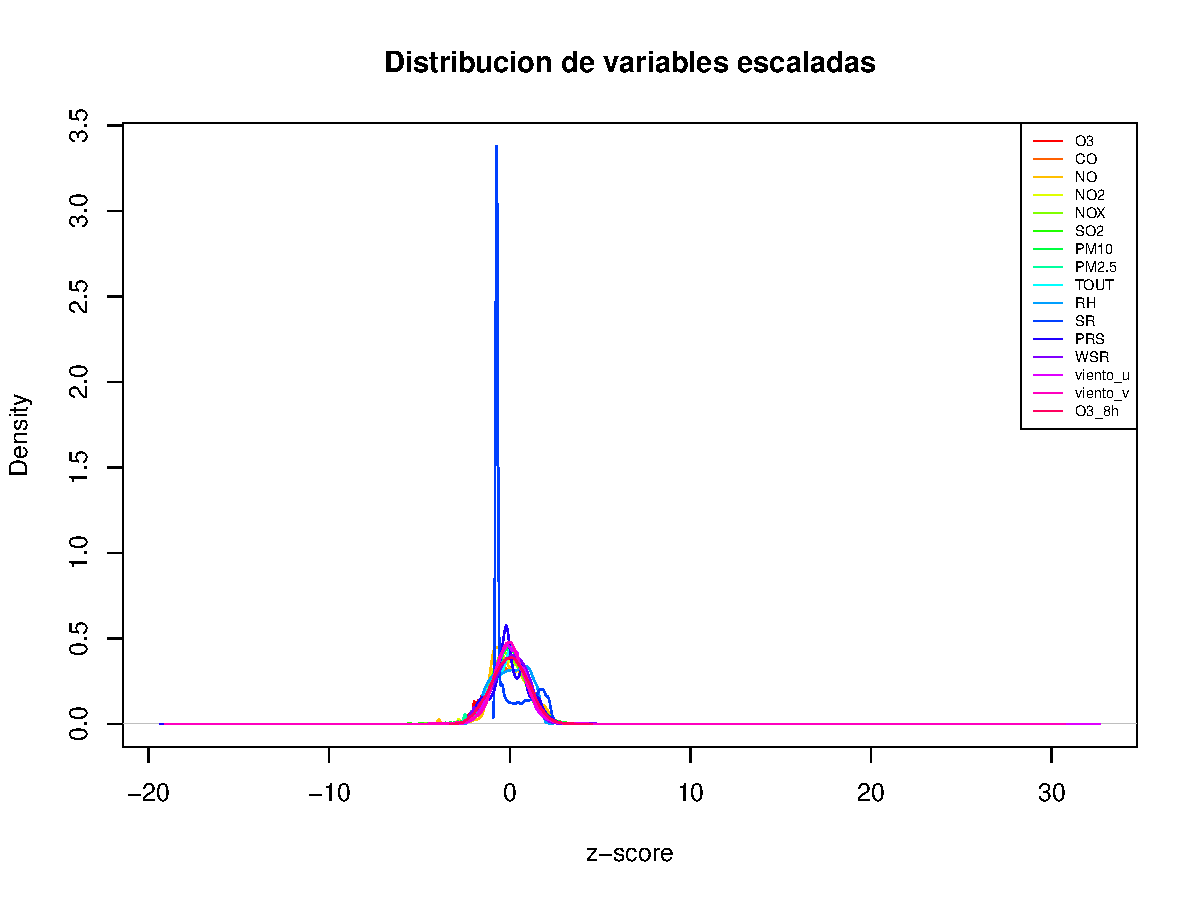
\includegraphics[width=\linewidth]{densidad_variables_escaladas.pdf}
  \caption{Distribution (density) of the quantitative variables after the
    Box-Cox transformation and scaling.}
  \label{fig:densidad-escaladas}
\end{figure}

The dictionary of the transformed dataset, with the full description of each
variable, its treatment and its skewness before and after, is given in
\cref{sec:diccionario-transformado}.


\section{Exploratory analysis}
\label{sec:eda}

\subsection{Quantitative variables}

\subsubsection{Quartiles and outlier bounds}

The quartiles and $1.5\times$IQR bounds of the hourly variables are reported
in their original units (\cref{tab:cuartiles-iqr}) and are the same ones the
cleaning used as the outlier criterion. \texttt{RAINF} and \texttt{WDR} are
excluded: \texttt{WDR} is circular and \texttt{RAINF} is zero-inflated, so
their IQR cannot be interpreted as a bound (\cref{sec:dic:meteorologicos}).
Two readings matter for what follows: the median zonal wind component is
negative, that is, the prevailing wind enters from the east
(\cref{sec:contexto-estaciones}); and the upper bound of \texttt{O3\_8h}
(66.22 ppb) lies above the 51 ppb threshold, so exceedance is not an outlier
but part of the usual range of the variable.

\begin{table}[t]
  \centering
  \caption{Quartiles and outlier bounds ($1.5\times$IQR criterion) of the
    hourly quantitative variables, in their original units.}
  \label{tab:cuartiles-iqr}
  \small
  \begin{tabular}{lrrrr}
    \toprule
    Variable & Q1 & Q3 & Lower & Upper \\
    \midrule
    \texttt{O3}       &    13.00 &    37.00 &  $-23.00$ &    73.00 \\
    \texttt{CO}       &     0.71 &     1.83 &   $-0.96$ &     3.50 \\
    \texttt{NO2}      &     6.90 &    19.70 &  $-12.30$ &    38.90 \\
    \texttt{NOX}      &    10.95 &    30.70 &  $-18.68$ &    60.33 \\
    \texttt{PM10}     &    35.00 &    74.00 &  $-23.50$ &   132.50 \\
    \texttt{PM2.5}    &    10.00 &    26.74 &  $-15.11$ &    51.85 \\
    \texttt{TOUT}     &    18.49 &    28.39 &      3.64 &    43.24 \\
    \texttt{PRS}      &   709.70 &   721.70 &    691.70 &   739.70 \\
    \texttt{WSR}      &     4.70 &    11.60 &   $-5.65$ &    21.95 \\
    \texttt{O3\_8h}   &    15.44 &    35.75 &  $-15.03$ &    66.22 \\
    \texttt{viento\_u}&  $-8.56$ &     0.21 &  $-21.73$ &    13.37 \\
    \texttt{viento\_v}&  $-3.38$ &     3.98 &  $-14.41$ &    15.01 \\
    \bottomrule
  \end{tabular}
\end{table}

\Cref{fig:boxplot-medidas} shows the distribution of each variable in
original units. All pollutant concentrations have a long right tail, with
outliers several times the third quartile; this is the asymmetry that
motivated Box-Cox in \cref{sec:transformaciones}. The meteorological
variables are more symmetric, except wind speed.

\begin{figure}[t]
    \centering
    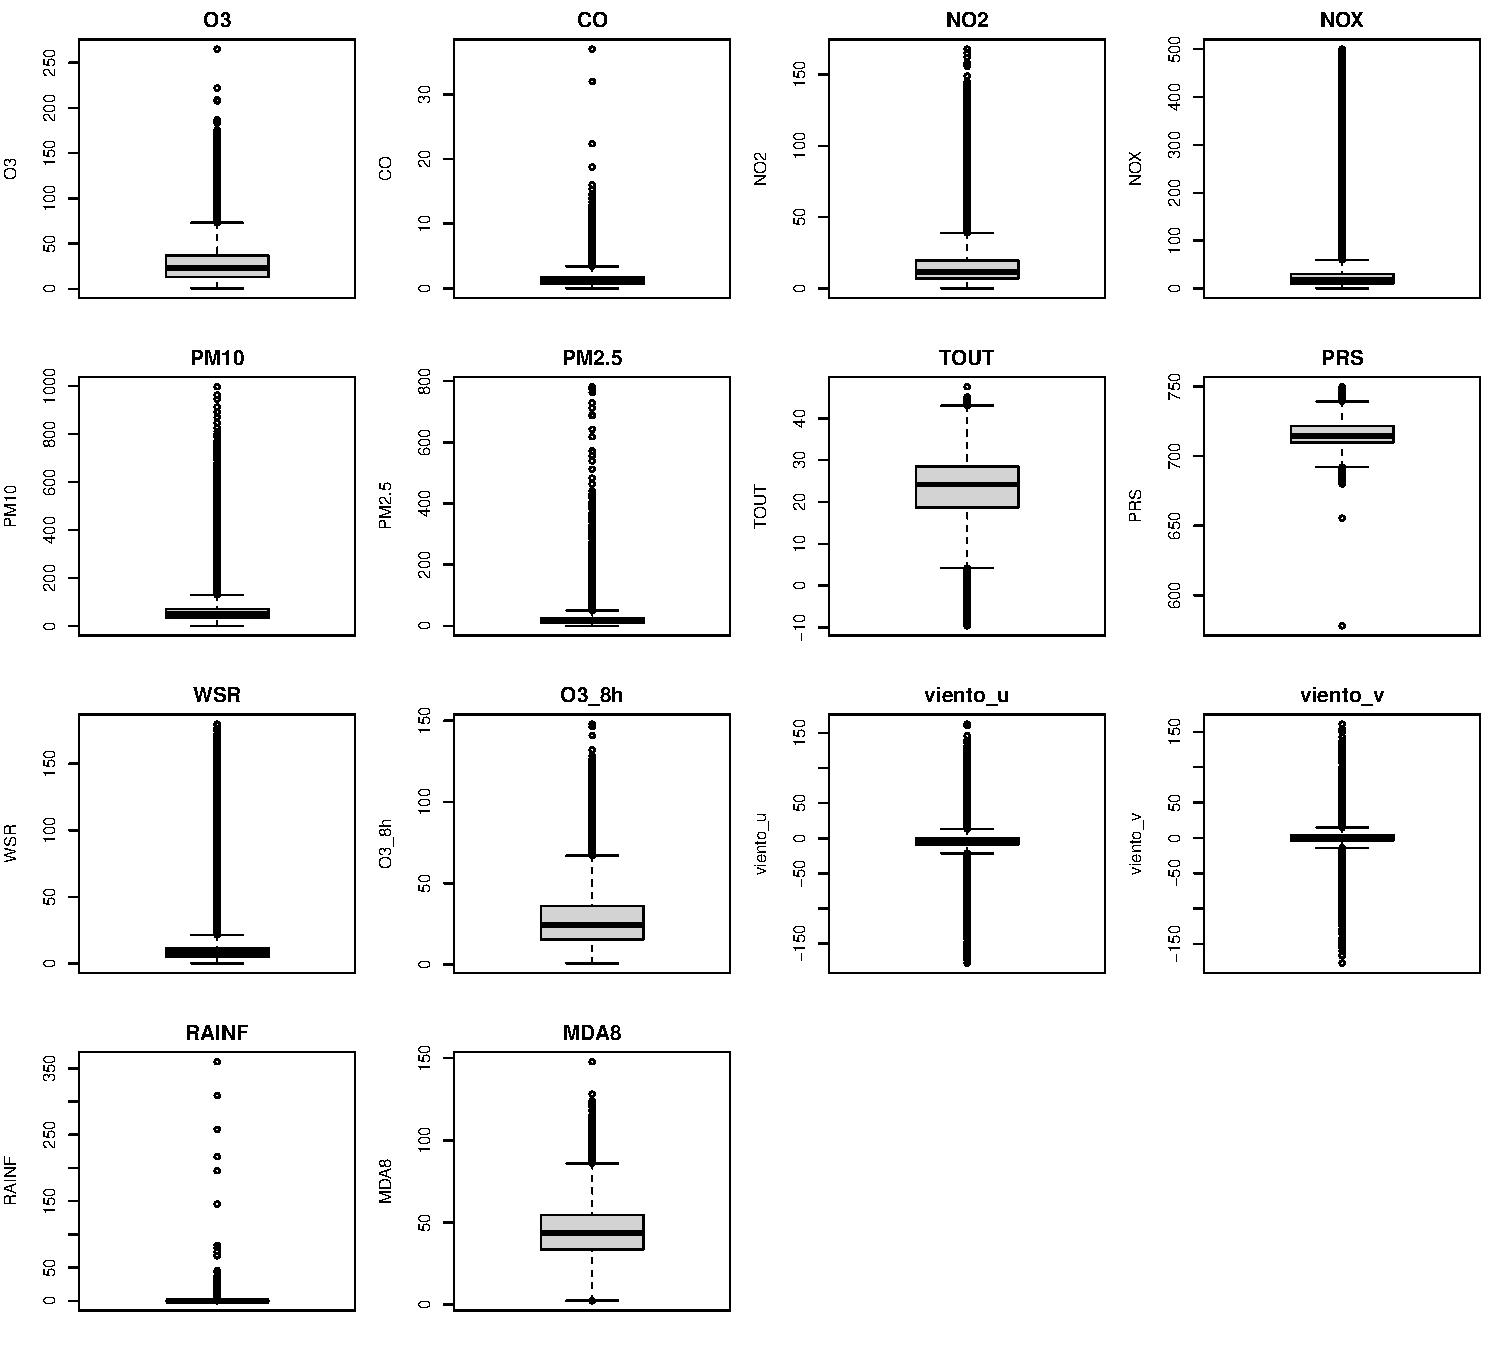
\includegraphics[width = \linewidth]{boxplots_medidas.pdf}
    \caption{Box plots of each hourly quantitative variable, in original
      units.}
    \label{fig:boxplot-medidas}
\end{figure}

\subsubsection{Correlation}

At hourly resolution and on the transformed scale, the strongest pairs are
\texttt{NO2}--\texttt{NOX} ($r=0.89$), the expected multicollinearity between
precursors of the same reaction cycle; \texttt{O3}--\texttt{O3\_8h}
($r=0.69$), by construction; \texttt{PM10}--\texttt{PM2.5} ($r=0.62$),
particulate matter of common origin; \texttt{O3}--\texttt{TOUT} ($r=0.52$)
and \texttt{O3}--\texttt{WSR} ($r=0.43$), consistent with the photochemical
mechanism; and \texttt{O3}--\texttt{NOX} ($r=-0.43$), which reflects the
consumption of \ce{O3} by titration with \ce{NO} near traffic sources.

PCA runs on the daily table and requires its own matrix: aggregating to days
changes the sample size and typically increases correlations by cancelling
measurement noise. It is computed over the 16 continuous variables of the
transformed daily dataset, on the subset with all 16 simultaneously complete
($n=15{,}856$ of 26,691 station-days, 59.4\,\%), the same listwise deletion
rule used in modeling, which guarantees a positive semidefinite matrix
(\cref{fig:mapa-calor-diario}).

\begin{figure}[t]
    \centering
    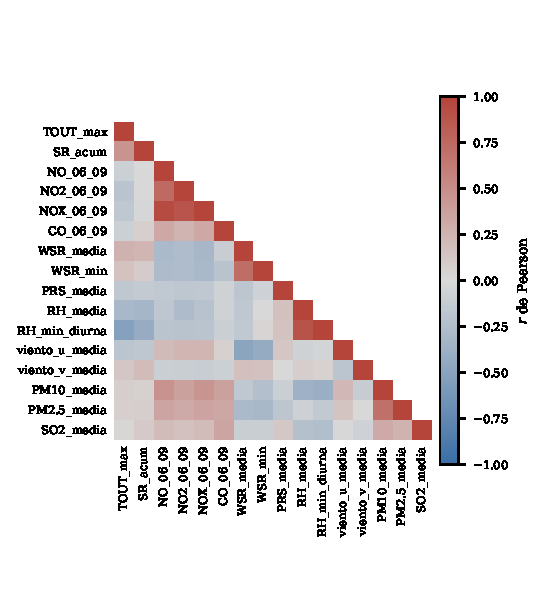
\includegraphics[width = \linewidth]{mapa_calor_correlacion_diario.pdf}
    \caption{Pearson correlation heat map of the 16 continuous variables of
      the transformed daily dataset, $n=15{,}856$ complete station-days.}
    \label{fig:mapa-calor-diario}
\end{figure}

Three hourly pairs have a direct analogue in the daily dataset:
\texttt{NO2}--\texttt{NOX} is unchanged (0.89), \texttt{PM10}--\texttt{PM2.5}
rises to 0.70, and \texttt{viento\_u}--\texttt{WSR} increases in magnitude to
$-0.48$. The ordering does change: \texttt{NO}--\texttt{NOX} ($r=0.95$) and
\texttt{RH\_media}--\texttt{RH\_min\_diurna} ($r=0.89$) dominate, absent from
the hourly map because \texttt{NO} and \texttt{RH} were not part of that set.
The first is the definitional redundancy \texttt{NOX} $\approx$ \texttt{NO} +
\texttt{NO2}; the second, and also \texttt{WSR\_media}--\texttt{WSR\_min}
($r=0.71$), is the same variable summarized twice over different windows of
the day. These construction redundancies are the ones that factor analysis
(\cref{sec:analisis-factorial}) eventually removes.

The diagnostics prior to PCA confirm the multicollinearity
(\cref{tab:diagnostico-pca}): the determinant is close to 0 and the condition
number is high. Bartlett's test of sphericity rejects that the matrix is the
identity ($\chi^2(120)=169{,}140.7$, $p<0.001$), and the overall KMO clears
the conventional threshold of 0.6; at the variable level, \texttt{RH\_media}
(0.587), \texttt{PRS\_media} (0.589) and \texttt{TOUT\_max} (0.596) fall just
below it without pulling down the total. The four diagnostics justify
applying PCA to the daily predictors.

\begin{table}[t]
  \centering
  \caption{Diagnostics prior to PCA on the daily correlation matrix
    ($n=15{,}856$, 16 variables).}
  \label{tab:diagnostico-pca}
  \small
  \begin{tabular}{lr}
    \toprule
    Diagnostic          & Value \\
    \midrule
    Determinant         & $2.32\times10^{-5}$ \\
    Condition number    & 322.8 \\
    Overall KMO         & 0.660 \\
    \bottomrule
  \end{tabular}
\end{table}

\subsection{Qualitative variables}
\label{sec:eda-cualitativas}

The categorical variables are reported in two blocks by unit of analysis:
\texttt{periodo} (period of the day) and \texttt{llovio} exist only at
hourly resolution; the exceedance indicators derive from the MDA8 and exist
only at daily resolution. Mixing them would replicate each daily value 24
times. The bases are $n = 640{,}583$ station-hour records and
$n = 26{,}691$ station-days.

\subsubsection{Frequency distribution}

\Cref{tab:freq-horaria} gathers the hourly variables. With 2025 complete, the
four seasons are balanced (24.79\,\% to 25.16\,\%), so no seasonal contrast is
an artifact of the observation window. \texttt{periodo} is uniform by
construction: four 6-hour blocks over a complete hourly grid.
\texttt{llovio} is the only hourly variable with missing data (19,360
records, 3.02\,\%), which are kept as a separate category rather than
assigned to ``did not rain''; it rains in 1.49\,\% of the hours with a
measurement. \texttt{tipo\_dia} replaces the weekend dummy because it
separates Saturday from Sunday, whose traffic patterns differ, and isolates
the 81 public holidays of the period.

\begin{table}[t]
  \centering
  \caption{Absolute and relative frequency of the qualitative variables at
    station-hour resolution ($n = 640{,}583$). Percentages are over records
    with valid data.}
  \label{tab:freq-horaria}
  \small
  \begin{tabular}{llrr}
    \toprule
    Variable & Level & Frequency & \% \\
    \midrule
    \multirow{4}{*}{\texttt{temporada}}
                                  & Winter    &   158,783 &  24.79 \\
                                  & Spring    &   161,184 &  25.16 \\
                                  & Summer    &   161,184 &  25.16 \\
                                  & Autumn    &   159,432 &  24.89 \\
    \midrule
    \multirow{4}{*}{\texttt{periodo}}
                                  & Early morning &   160,145 &  25.00 \\
                                  & Morning   &   160,146 &  25.00 \\
                                  & Afternoon &   160,146 &  25.00 \\
                                  & Night     &   160,146 &  25.00 \\
    \midrule
    \multirow{4}{*}{\texttt{tipo\_dia}}
                                  & Weekday   &   434,879 &  67.89 \\
                                  & Saturday  &    88,392 &  13.80 \\
                                  & Sunday    &    88,728 &  13.85 \\
                                  & Holiday   &    28,584 &   4.46 \\
    \midrule
    \multirow{3}{*}{\texttt{llovio}}
                                  & No (0)    &   611,952 &  98.51 \\
                                  & Yes (1)   &     9,271 &   1.49 \\
                                  & Missing   &    19,360 &    --- \\
    \bottomrule
  \end{tabular}
\end{table}

\Cref{tab:freq-diaria} presents the daily block. The three MDA8 indicators
share the same 1,591 missing records (5.96\,\%), the station-days whose MDA8
did not reach the completeness of 18 of 24 windows; \texttt{excede\_1h} does
not share them because it is computed on the hourly maximum.

\begin{table}[t]
  \centering
  \caption{Absolute and relative frequency of the exceedance indicators at
    station-day resolution ($n = 26{,}691$; valid $= 25{,}100$ for the MDA8
    indicators).}
  \label{tab:freq-diaria}
  \small
  \begin{tabular}{llrr}
    \toprule
    Variable & Level & Frequency & \% \\
    \midrule
    \multirow{3}{*}{\texttt{excede\_anio\_1} (65 ppb)}
                                        & No        &  22,275 &  88.75 \\
                                        & Yes       &   2,825 &  11.25 \\
                                        & Missing       &   1,591 &    --- \\
    \midrule
    \multirow{3}{*}{\texttt{excede\_anio\_3} (60 ppb)}
                                        & No        &  20,864 &  83.12 \\
                                        & Yes       &   4,236 &  16.88 \\
                                        & Missing       &   1,591 &    --- \\
    \midrule
    \multirow{3}{*}{\texttt{excede\_anio\_5} (51 ppb)}
                                        & No        &  17,079 &  68.04 \\
                                        & Yes       &   8,021 &  31.96 \\
                                        & Missing       &   1,591 &    --- \\
    \midrule
    \multirow{2}{*}{\texttt{excede\_1h} (90 ppb)}
                                        & No        &  24,497 &  91.78 \\
                                        & Yes       &   2,194 &   8.22 \\
    \bottomrule
  \end{tabular}
\end{table}

\subsubsection{The monitoring station}

Fourteen of the 15 stations record 43,824 observations each, the complete
hourly grid from 2021-01-01 to 2025-12-31; \texttt{NO3} records 27,047
because it started operating on 1 December 2022. The difference is one of
coverage, not quality: within its window, \texttt{NO3} also has a complete
grid, and its share of hours with measured \ce{O3} is within the range of the
rest of the network. \texttt{periodo}, the only ordinal variable, has median
\texttt{tarde} (afternoon) over the 611,601 hours with measured \ce{O3},
because missing data concentrate at night.

\subsubsection{Class balance}

\Cref{fig:eda-cual-excedencias} shows the balance of the three MDA8
indicators. At the current 65 ppb threshold, exceedances are 11.25\,\% of
valid station-days: a classifier that always predicts the majority class
reaches 88.75\,\% accuracy without capturing the phenomenon, so accuracy is
discarded as a metric in favor of sensitivity, specificity and area under
the ROC curve. The 51 ppb threshold, with 31.96\,\%, offers a substantially
better balance and is the main modeling scenario.

\begin{figure}[t]
  \centering
  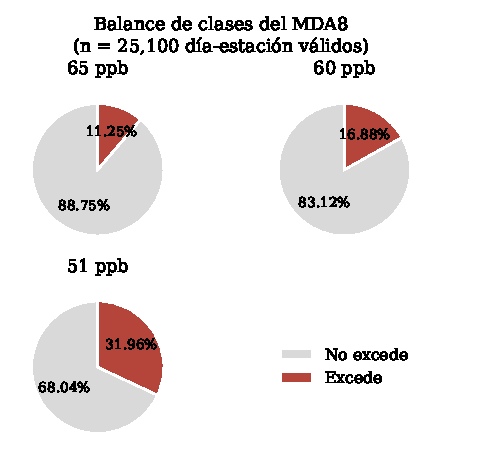
\includegraphics[width=\linewidth]{eda_cual_excedencias.pdf}
  \caption{Class balance of the MDA8 exceedance indicators for the three
    gradual compliance thresholds of NOM-020-SSA1-2021
    (\cref{tab:nom-limites}).}
  \label{fig:eda-cual-excedencias}
\end{figure}


\section{Modeling and validation}
\label{sec:modelacion}

All techniques share the same temporal partition: the years 2021--2024 are
used for fitting and the full year 2025 for validation. The rule is strict:
no procedure sees 2025 during fitting, including PCA and FA, whose axes are
estimated on 2021--2024 and applied to 2025 with the training weights;
otherwise information from the validation partition would leak into the
coordinates consumed by the classifiers. The only remaining leak is the
Box-Cox parameter $\lambda$, estimated on the full period in
\cref{sec:transformaciones}; it is declared because reverting it would
require rebuilding the transformed dataset.

Validation has a particularity that runs through all the results: 2025 is the
year with the highest ozone in the series, with 44.0\,\% station-day
exceedance versus 29.4\,\% in the fitting period, in all four seasons. It is
a year effect, not a calendar effect, and each technique revisits it where it
matters.

The five techniques are presented in the order in which each feeds the next:
PCA (\cref{sec:pca}) and FA (\cref{sec:analisis-factorial}) reduce the
15 predictors to three axes; the time-series characterization
(\cref{sec:serie-tiempo}) establishes the temporal dependence of those axes;
logistic regression and the discriminant (\cref{sec:clasificacion_tecs})
classify the station-day; and the autoregressive model
(\cref{sec:autorregresivo}) incorporates temporal dependence into the
classification.

\subsection{Principal component analysis}
\label{sec:pca}

PCA is needed to handle the multicollinearity of the predictors before they
enter the models: \texttt{NO} and \texttt{NOX} correlate at 0.95. The
expected outcome is a set of principal components with names that are
interpretable in context, together with the structure of their loadings. The
procedure is applied to the station-day data. The categorical variables
(\texttt{tipo\_dia}, \texttt{temporada}, \texttt{festivo}, \texttt{zona}) are
excluded, as are the variables derived from \texttt{O3} and the exceedance
indicators: these are the response, and using them would leak information,
building components that contain what is meant to be predicted. Of the 16
continuous daily variables, \texttt{PM2.5} is also excluded, because station
\texttt{NE3} does not measure it and listwise deletion would remove that
station entirely; its signal is largely carried by \texttt{PM10} ($r=0.70$).
PCA therefore runs on 15 predictors.

It is fitted on 2021--2024 only and applied to 2025 (\cref{sec:modelacion}).

The eigenvalues are computed and the scree plot is built
(\cref{fig:scree_pca}); the number of components to retain is set by the
elbow method. The curvature places the cut at the third principal component.

The loadings are the product of the eigenvectors and the square root of the
corresponding eigenvalues, so they are interpreted as the correlation between
the variables and the components (\cref{tab:pca-cargas}).

The first component has high loadings on \texttt{NOX}, \texttt{NO2},
\texttt{NO} and \texttt{PM10}, and a negative loading on \texttt{WSR\_min}
($-0.48$). These variables are mainly the substances that take part in the
chemical reactions that form ozone, whose main source is the burning of
fossil fuels, while wind speed (with a negative loading) acts as dispersion;
for this reason \texttt{PC1} is named \textit{primary combustion load}.

\texttt{PC2} has high negative loadings on relative humidity and high
positive loadings on solar radiation and temperature. These variables are
related: as temperature rises, relative humidity falls, since warm air can
hold more water vapor, and sunnier, drier days increase ozone production.
This component is \textit{photochemical forcing}.

The third component gathers the conditions that affect the stagnation of
pollutants: higher pressure increases stagnation, and higher wind speed
reduces it. This component is \textit{atmospheric stagnation}
(\cref{fig:pca_biplot}).

The three components account for 55.9\,\% of the variance of the 15
predictors. The benchmark for that figure is not 100\,\% but what three
components would produce on independent variables: with $p = 15$ each
eigenvalue would equal 1 and three would account for 20\,\%. The retained
eigenvalues are 3.92, 2.97 and 1.50, 2.8 times the null. The correlation
between \texttt{NO} and \texttt{NOX} that motivated the analysis is absorbed
into \texttt{PC1}, and the three coordinates inherited by the subsequent
models are orthogonal by construction. The mean 2025 scores are not zero
(\texttt{PC1} $-0.39$, \texttt{PC3} $+0.35$): 2025 has less primary load and
more stagnation than the 2021--2024 average, the year effect of
\cref{sec:modelacion}, not a fitting error.

\begin{figure}[t]
  \centering
  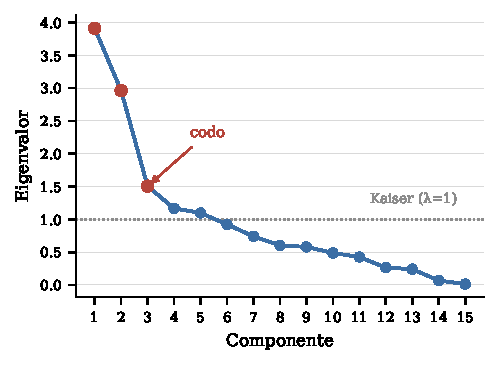
\includegraphics[width = \linewidth]{pca_scree.pdf}
  \caption{Variance explained by each component. The largest drop occurs at
    the third component; beyond it the gain is marginal.}
  \label{fig:scree_pca}
\end{figure}

\begin{table}[ht]
  \centering
  \caption{Dominant loadings of the retained components, with the variance
    explained by each.}
  \label{tab:pca-cargas}
  \begin{tabular}{lr}
    \toprule
    Component and variable & Loading \\
    \midrule
    \multicolumn{2}{l}{\emph{Primary combustion load} (26.1\,\%)} \\
    \quad \texttt{NOX}      & 0.88 \\
    \quad \texttt{NO}       & 0.82 \\
    \quad \texttt{NO2}      & 0.81 \\
    \quad \texttt{PM10}     & 0.66 \\
    \quad \texttt{WSR\_min} & $-0.48$ \\
    \midrule
    \multicolumn{2}{l}{\emph{Photochemical forcing} (19.8\,\%)} \\
    \quad \texttt{RH\_min\_diurna} & $-0.77$ \\
    \quad \texttt{TOUT\_max}       & 0.72 \\
    \quad \texttt{RH\_media}       & $-0.70$ \\
    \quad \texttt{SR\_acum}        & 0.64 \\
    \quad \texttt{WSR\_media}      & 0.61 \\
    \midrule
    \multicolumn{2}{l}{\emph{Atmospheric stagnation} (10.0\,\%)} \\
    \quad \texttt{WSR\_min}        & $-0.50$ \\
    \quad \texttt{viento\_u\_media} & 0.48 \\
    \quad \texttt{WSR\_media}      & $-0.41$ \\
    \quad \texttt{PRS\_media}      & 0.40 \\
    \quad \texttt{RH\_min\_diurna} & $-0.37$ \\
    \bottomrule
  \end{tabular}
\end{table}

\begin{figure}[t]
  \centering
  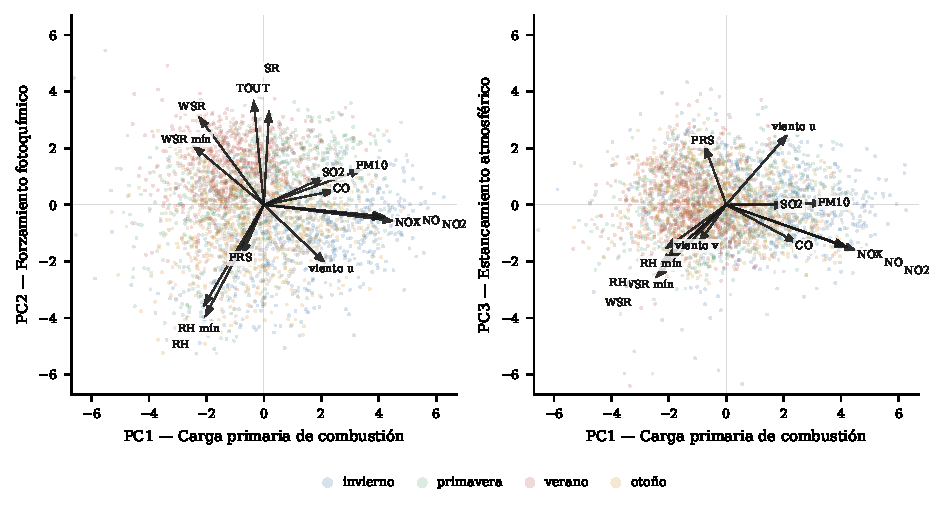
\includegraphics[width = \linewidth]{pca_biplot.pdf}
  \caption{Biplot of the retained axes. Points: subsample of 3,000 training
    observations, colored by season. Arrows: loadings scaled to the frame.
    Abbreviated names: \texttt{TOUT} and \texttt{SR} are the daily maximum
    and total; \texttt{NO}, \texttt{NO2}, \texttt{NOX} and \texttt{CO} are
    the 06--09 h window; the rest are daily means, except \texttt{WSR} min
    and \texttt{RH} min.}
  \label{fig:pca_biplot}
\end{figure}

\subsection{Exploratory factor analysis}
\label{sec:analisis-factorial}

Factor analysis complements PCA (\cref{sec:pca}) by separating the variance
shared among variables from the variance specific to each. For each
standardized variable,
\begin{equation}
  z_j=\sum_{k=1}^{3}\lambda_{jk}f_k+\varepsilon_j,
  \qquad h_j^2=\sum_{k=1}^{3}\lambda_{jk}^2.
  \label{eq:af-modelo}
\end{equation}
The $f_k$ are latent factors, and the loadings $\lambda_{jk}$ give the
magnitude and direction of their association with each variable. With
orthogonal factors of unit variance, the communality $h_j^2$ is the
proportion of variance explained; the uniqueness $1-h_j^2$ captures the
specific part and the error.

\paragraph{Adequacy and extraction}
The initial diagnosis uses 15 predictors and 16,028 complete observations
from 2021--2024. Bartlett's test rejects the absence of correlations
($p<0.001$), although temporal and spatial dependence limit this test. The
initial KMO of 0.647 indicates mediocre adequacy. \texttt{NOX\_06\_09} is
removed because of its redundancy with NO and NO2 (VIF of 45.73). On the
remaining 14 variables, Velicer's MAP suggests three factors, versus seven
from parallel analysis; MAP is adopted for parsimony, and the discrepancy is
kept as a limitation.

Iterated principal axis extraction produces an inadmissible communality of
1.093 for \texttt{RH\_min\_diurna}; this variable is removed and mean
humidity is kept. The final block of 13 predictors reaches a KMO of 0.677
and a maximum VIF of 2.54, with no communalities above one. Three factors are
retained and varimax is applied to ease their interpretation through
orthogonal axes (\cref{fig:af-diagrama}).

\begin{figure}[pos=t]
  \centering
  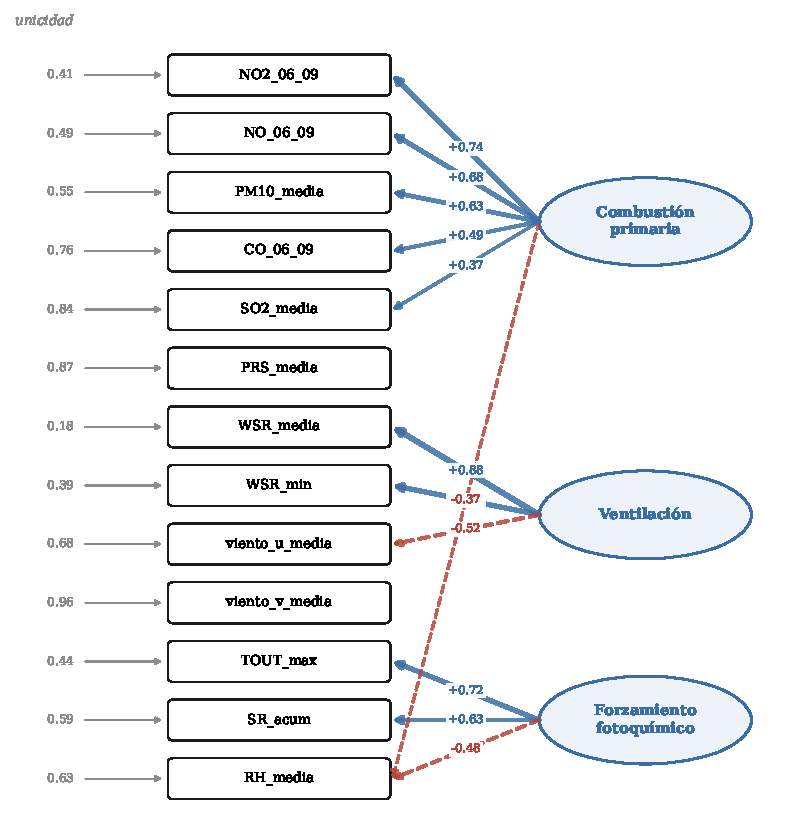
\includegraphics[width=0.92\linewidth]{af_diagrama_cargas.pdf}
  \caption{Varimax loadings with $|\lambda|\geq0.30$. Solid arrows: positive
    associations; dashed: negative. Gray values indicate uniquenesses.}
  \label{fig:af-diagrama}
\end{figure}

\paragraph{Interpretation}
The factors explain 40.3\,\% of the total variance of the 13 predictors.
\emph{Primary combustion} (15.7\,\%) groups NO2 (0.74), NO (0.68), PM10
(0.63), CO (0.49) and SO2. \emph{Ventilation} (14.5\,\%) gathers mean and
minimum wind speed, with loadings of 0.88 and 0.77, and the zonal component
($-0.52$). \emph{Photochemical forcing} (10.1\,\%) combines maximum
temperature (0.72), cumulative radiation (0.63) and mean humidity ($-0.48$):
warm, sunny, dry days. Pressure has a communality of only 0.13, so the name
ventilation is more accurate than attributing an anticyclonic mechanism to
the factor.

Three choices that were tried and discarded along the way ---Horn's parallel
analysis, maximum likelihood extraction and oblique rotation--- are
documented in \cref{sec:tecnicas-descartadas}.

\paragraph{Fit and scope}
The root mean square residual of the reconstructed correlations (RMSR) is
0.0555; 26 of 78 pairs retain absolute residuals greater than 0.05. The fit
is reasonable but partial. Bartlett scores, applied to 2025 with training
weights, have VIFs close to 1.01 and a maximum absolute correlation of 0.097.
That is why they, rather than the PCA scores, are the predictors of the
models of \cref{sec:clasificacion_tecs}, where the comparison is reported.

The three factors reappear in 2025 with Tucker congruence coefficients of
0.973 for combustion, 0.939 for ventilation and 0.924 for photochemistry: the
structure is stable outside the fitting period. The factor score determinacy
(correlation between score and factor) is 0.880, 0.918 and 0.833;
photochemical forcing shares 69\,\% of its variance with the factor it
represents, and the rest is estimation error. The mediocre KMO and the
Box--Cox transformation estimated on the full period remain as caveats. The
factors describe associations; without measurements of volatile organic
compounds they cannot establish ozone formation mechanisms.

\subsection{Time series of the factor scores and exceedance}\label{sec:serie-tiempo}

The response \texttt{excede\_anio\_5} (\cref{sec:obj:objetivo}) and the
three factor scores of \cref{sec:analisis-factorial} are characterized here
over time: their origin and validity, already established, are not
revisited, only their behavior as series.

\subsubsection{From station-day to metropolitan area}

Any time-series decomposition requires a series without gaps, and the
station-day panel is not one. Only 2 of the 15 stations (\texttt{CE},
\texttt{SE3}) exceed 85\,\% coverage of valid station-days over the
2021--2025 calendar, and the worst, \texttt{NO3}, reaches 25\,\%; overall
coverage is 68.0\,\%. Filtering to the best-covered stations does not solve
the problem, it hides it in the three that survive the cut.

The alternative is to aggregate the 15 stations into a daily
metropolitan-area value, which is only reasonable if stations are not
independent of one another on the same day. The cross-sectional correlation
(Pearson, station against station, same day) ranges from a mean of 0.50 for
ventilation to 0.85 for photochemical forcing, with a barely negative
minimum only for ventilation. This is consistent with the physics:
temperature and solar radiation are regional-scale phenomena, whereas wind
depends on the local topography of the valley. This correlation is also the
largest violation of independence in the dataset, relevant to any model that
treats each station-day row as an observation ---including the
autocorrelation limitation already declared in
\cref{sec:limitaciones-clasificacion}.

Given the insufficient coverage per station and the high cross-sectional
correlation, the data are aggregated at the metropolitan-area level by
averaging the stations that report each day. The average recovers
99.94\,\% coverage of the daily calendar; a single day, 2021-02-16, has no
station at all and is imputed by linear interpolation ---only because the
MSTL decomposition requires a series without gaps, not because the gap
ceases to exist.

\subsubsection{MSTL decomposition}

MSTL is fitted with weekly (7) and annual (365, not 365.25: MSTL requires
integer periods and the accumulated drift over 5 years is about one day,
negligible) periods to the four metropolitan-area series. The weekly cycle is
strongest for primary combustion ---the weekday/weekend pattern of traffic
and industrial activity--- and weakest for the fraction of stations above the
threshold, which dilutes that pattern because it depends on several factors
at once.

\subsubsection{Residual autocorrelation}

The Ljung-Box test at lags 7, 14 and 30 rejects with $p<0.001$ for all four
series, in both versions (raw and MSTL residual) ---the same problem that
\cref{sec:analisis-factorial} noted for Bartlett: with $n=1{,}826$ daily
observations, the statistic grows with $n$ and rejects any non-trivial
autocorrelation, including that of the residual, where seasonality has
already been removed. The test does not discriminate; the magnitude of the
ACF does (\cref{fig:acf-excedencia}).

\begin{figure}[t]
  \centering
  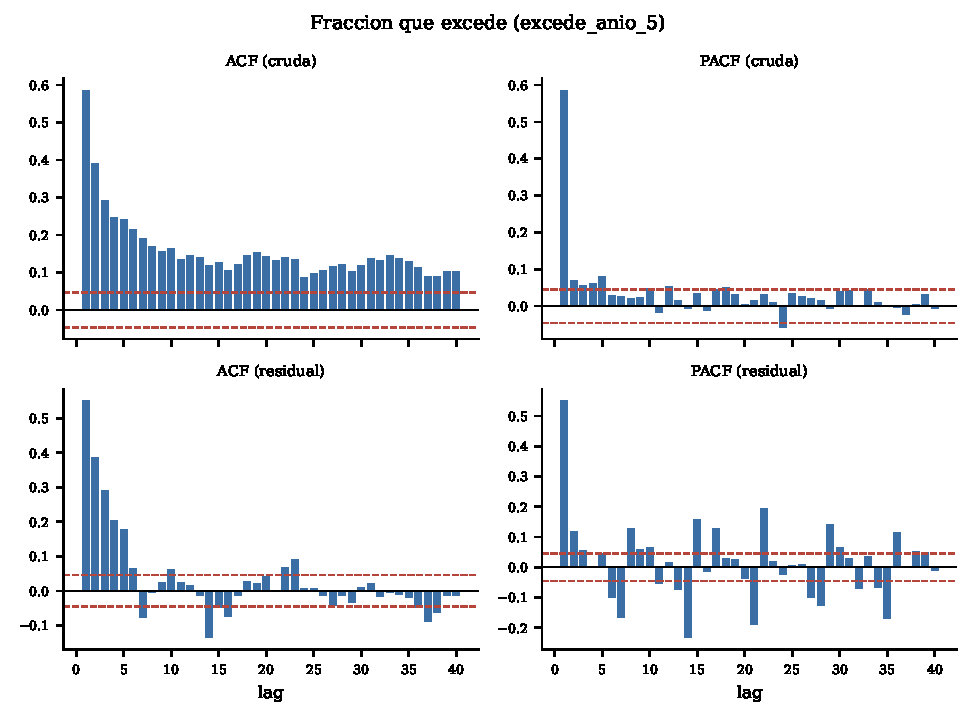
\includegraphics[width=\linewidth]{acf_pacf_frac_excede_anio_5.pdf}
  \caption{ACF and PACF up to lag 40 of the exceeding fraction: raw series
    (top) versus MSTL decomposition residual (bottom), with
    $\pm 1.96/\sqrt{n}$ band.}
  \label{fig:acf-excedencia}
\end{figure}

After MSTL, the lag-7 autocorrelation falls from 0.19--0.45 to values between
$-0.15$ and 0.05 in the four series ---the weekly seasonality practically
disappears. The lag-1 autocorrelation, by contrast, remains between 0.49 and
0.71 in the residual of all four series. That day-to-day persistence is not
seasonality: it is genuine short-term autocorrelation, which MSTL is not
designed to remove. It quantifies, with a continuous series without gaps, the
same temporal dependence that \cref{sec:limitaciones-clasificacion} identified
as the reason the standard errors of the logistic model are optimistic.

Two consequences carry over to the autoregressive model of
\cref{sec:autorregresivo}: lags must be computed on the metropolitan-area
series reindexed to a regular daily calendar, never on the station-day
table, where the previous row may be a week away; and the day-to-day
dependence is genuine, not an artifact of seasonality, so a model that
ignores it leaves structure in the residuals.
%
\subsection{Classification: logistic regression and discriminant analysis}
\label{sec:clasificacion_tecs}

The factor scores of \cref{sec:analisis-factorial} are joined by station and
date with the categorical variables of the station-day and with the response
\texttt{excede\_anio\_5}. The scores do not have unit variance (standard
deviations of 1.14, 1.10 and 1.21 in the fitting period), so they are
rescaled with the mean and standard deviation of 2021--2024, never with those
of 2025; each odds ratio is then read per standard deviation of the factor,
and the three are comparable with one another. The categorical variables
\texttt{zona}, \texttt{tipo\_dia} and \texttt{temporada} enter as 12
indicators against the reference levels Northeast, weekday and winter. The
design matrix has 15 predictors; 16,058 rows enter the fit and 2,978 the
validation.

\subsubsection{Logistic regression}\label{sec:reg_log}

The model is fitted on 2021--2024 only. The odds ratios are reported in
\cref{tab:momios-log}; no interval for the three factors crosses 1.
Photochemical forcing has the largest effect: one additional standard
deviation multiplies the odds of exceedance by 2.78, versus 1.92 for primary
combustion. The reading is chemical: precursors are necessary, but the rate
and volume of the reactions that produce ozone depend on temperature and
radiation, so the photochemical condition weighs more than the availability
of ingredients. Ventilation is the only protective factor (0.90): wind
disperses.

\begin{table}[pos=t]
  \centering
  \caption{Odds ratios of the logistic model (\texttt{exp} of the
    coefficient) with 95\,\% interval under independence. Factors are
    interpreted per standard deviation; indicators, against their reference
    level: Northeast (zone), weekday (\texttt{tipo\_dia}) and winter
    (\texttt{temporada}). All coefficients are significant ($p<0.001$)
    except \texttt{tipo\_dia\_sabado} ($p=0.04$) and
    \texttt{tipo\_dia\_festivo} ($p=0.13$).}
  \label{tab:momios-log}
  \small
  \begin{tabular}{lrc}
    \toprule
    Variable & Odds ratio & 95\,\% CI \\
    \midrule
    Primary combustion      & 1.92 & [1.82, 2.02] \\
    Ventilation             & 0.90 & [0.86, 0.95] \\
    Photochemical forcing   & 2.78 & [2.62, 2.94] \\
    \midrule
    \texttt{zona\_Centro}    & 2.74 & [2.32, 3.22] \\
    \texttt{zona\_Noroeste}  & 3.84 & [3.32, 4.43] \\
    \texttt{zona\_Norte}     & 1.76 & [1.50, 2.06] \\
    \texttt{zona\_Sur}       & 2.90 & [2.44, 3.44] \\
    \texttt{zona\_Sureste}   & 1.82 & [1.59, 2.09] \\
    \texttt{zona\_Suroeste}  & 3.48 & [3.02, 4.01] \\
    \midrule
    \texttt{tipo\_dia\_sabado}  & 1.13 & [1.01, 1.27] \\
    \texttt{tipo\_dia\_domingo} & 1.43 & [1.27, 1.62] \\
    \texttt{tipo\_dia\_festivo} & 1.17 & [0.95, 1.44] \\
    \midrule
    \texttt{temporada\_primavera} & 3.54 & [3.08, 4.08] \\
    \texttt{temporada\_verano}    & 1.54 & [1.31, 1.83] \\
    \texttt{temporada\_otono}     & 3.04 & [2.66, 3.49] \\
    \bottomrule
  \end{tabular}
\end{table}

The zones with the highest odds are Northwest (3.84) and Southwest (3.48):
for the same meteorology and calendar, the west of the city almost
quadruples the odds of the Northeast, the spatial ordering anticipated in
\cref{sec:contexto-estaciones}. Spring (3.54) and autumn (3.04) triple the
odds of winter, which, with lower temperature and radiation, slows the
photochemical reactions even when precursors are present; summer stays at
1.54. The working calendar has little influence: only Sunday (1.43) has a
clear effect.

\paragraph{Standard errors under dependence.} The 15 stations on the same day
share the weather, and consecutive days resemble each other, so standard
errors under independence are optimistic. They are corrected with the
sandwich estimator clustered by day (1,460 clusters): they inflate by
1.5 to 2.5 times, more for the calendar indicators, which are constant
within a day, and not at all for the zone indicators, which vary within it.
The corrected intervals of the three factors are almost twice as wide and
still do not cross 1 (\cref{fig:momios-corregido}): ventilation
$[0.84, 0.97]$, photochemical forcing $[2.48, 3.10]$. The only term that
loses significance at 5\,\% is Saturday. Clustering also by station is not
reliable with 15 clusters, but it makes clear that the six zone contrasts
rest on 15 units, not on 16,058 rows.

\begin{figure}[pos=t]
  \centering
  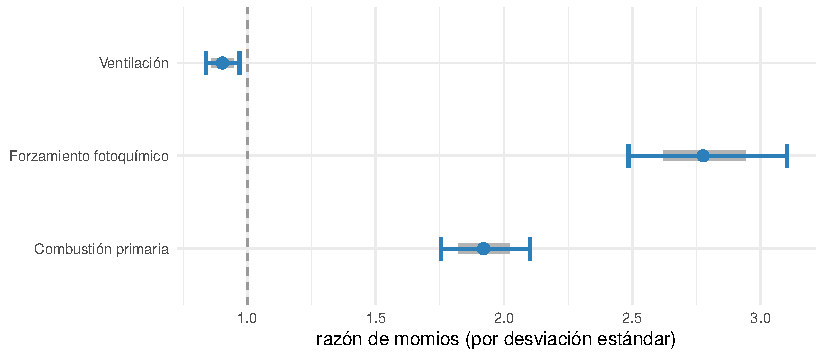
\includegraphics[width=\linewidth]{momios_ic_corregido.pdf}
  \caption{Odds ratios of the factors with 95\,\% intervals under
    independence (gray) and clustered by day (color). The corrected
    intervals are wider and none crosses 1.}
  \label{fig:momios-corregido}
\end{figure}

\paragraph{Evaluation and validation.} Evaluation is performed on 2025, not
seen during fitting, with AUC, sensitivity and specificity; accuracy is
discarded because the base exceedance rate in validation is 43.97\,\%. The
model reaches an AUC of 0.850 (\cref{fig:roc-modelos}), above the
performance threshold of 0.75. The classification threshold is chosen by
Youden's index on the fitting data and equals 0.282; at that threshold
sensitivity is 0.698 and specificity 0.853 (left panel of
\cref{fig:matrices}). A threshold of 0.5 illustrates why accuracy is not a
suitable criterion: specificity rises to 0.964, but sensitivity falls to
0.326, that is, the model misses two of every three actual exceedances.

\subsubsection{Linear discriminant analysis}\label{sec:lda}

The second technique is fitted on the same design matrix, the same response
and the same partition. The contrast is deliberate: the discriminant assumes
multivariate normality within each class and homoscedasticity between
classes, assumptions the logistic model does not require.

\paragraph{Checking assumptions.} The factor scores are linear combinations
of predictors with $|\text{skewness}|<0.5$ after Box-Cox. On the training
scores split by class, the six skewness coefficients lie between $-0.091$
and 0.489, so the normal approximation holds. Homoscedasticity does not: Box's
M test, which with more than 15,000 observations rejects arbitrarily small
differences, is not applied; instead, the class covariance matrices are
compared directly. Exceedance days are less dispersed than non-exceedance
days on all three factors, with standard deviation ratios of 0.894, 0.888
and 0.742, and the generalized variance drops from 1.081 to 0.346; the
discrepancy is concentrated on the photochemical axis. A second departure
affects the 12 binary indicators, which are not normal under any
transformation. Linear discriminant analysis tolerates both departures in
practice, and that tolerance is verified empirically in
\cref{sec:comparacion}.

\paragraph{Fit and evaluation.} The prior probabilities are set to the
proportions observed in the fitting period (0.706 and 0.294) because the base
rate is information about the problem. With two classes there is a single
discriminant function, and the order and sign of its coefficients reproduce
those of \cref{tab:momios-log}: photochemical forcing (0.795) dominates
primary combustion (0.506), ventilation works against exceedance ($-0.109$),
Northwest and Southwest are the highest-risk zones, and spring (1.054) and
autumn (0.772) weigh more than summer (0.176). The coefficients give the
direction of maximum separation between classes; they are not odds ratios.
Evaluation uses the posterior probability of exceedance as a continuous
score, so that the ROC curve is comparable with the logistic one. The
discriminant reaches an AUC of 0.846; at Youden's threshold (0.249)
sensitivity is 0.758 and specificity 0.788 (right panel of
\cref{fig:matrices}).

\subsubsection{Comparison of the two models}\label{sec:comparacion}

The two techniques are practically equivalent on these data: the AUCs differ
by three thousandths (0.850 versus 0.846), the scores correlate at 0.996, and
the classifications agree on 93.8\,\% of the validation station-days.
DeLong's test for correlated ROC curves does detect the difference
($Z=3.75$, $p=0.0002$, 95\,\% CI $[0.002, 0.005]$): with 2,927 observations
it has power for three thousandths, a statistically real difference with no
practical consequence. Where they do differ is in the distribution of errors
at Youden's threshold: the discriminant detects more exceedances
(sensitivity 0.758 versus 0.698) at the cost of more false alarms
(specificity 0.788 versus 0.853).

\begin{figure}[pos=t]
  \centering
  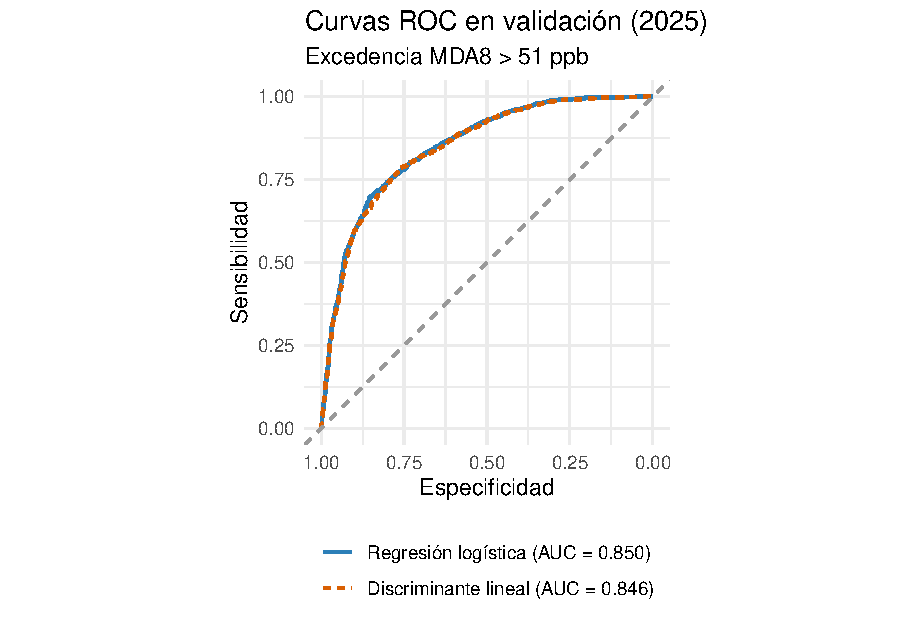
\includegraphics[width=\linewidth]{roc_modelos.pdf}
  \caption{ROC curves of both models on the validation partition (2025). The
    two curves overlap; the discriminant is drawn dotted.}
  \label{fig:roc-modelos}
\end{figure}

\begin{figure}[pos=t]
  \centering
  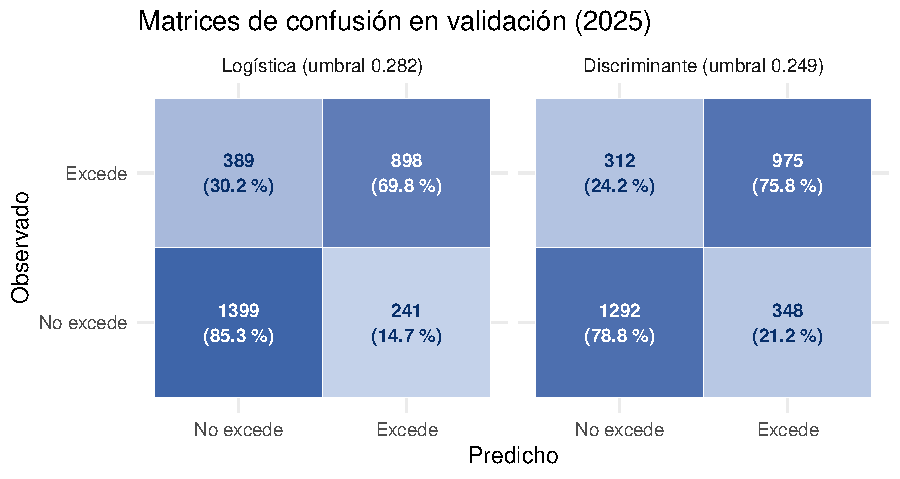
\includegraphics[width=\linewidth]{matriz_confusion.pdf}
  \caption{Confusion matrices in validation, each model at its own Youden
    threshold. Percentages are row proportions (observed class).}
  \label{fig:matrices}
\end{figure}

This agreement is the relevant result: the heteroscedasticity documented in
\cref{sec:lda} is real and still does not alter performance, so the decision
boundary drawn by both is the same, and the interpretation of the odds
ratios does not depend on the normality assumption that the discriminant
requires and the logistic model does not. As an additional contrast, the
logistic model on the PCA scores reaches an AUC of 0.848 (DeLong $p=0.44$
versus 0.850): the factors lose no discriminating power and gain
interpretability.

\paragraph{Error rate correction.} The apparent resubstitution error (0.229
for the logistic model, 0.230 for the discriminant) barely changes with
10-fold cross-validation by whole days (0.231 and 0.232) or with
Lachenbruch's method (0.231): with 16 parameters on 15,704 observations the
optimism is of order $p/n$, and neither classifier overfits. What
cross-validation does reveal is the year effect: within 2021--2024 the
out-of-sample AUC is 0.80, not 0.85. By year, each predicted by a model that
did not see it, 2021--2023 stay at 0.76--0.77, 2024 rises to 0.84 and 2025
to 0.85. The expected performance in an arbitrary year is 0.80; the 0.85
corresponds to the two high-ozone years.

\subsubsection{Limitations}\label{sec:limitaciones-clasificacion}

\textbf{Autocorrelation.} The 18,631 station-day rows of fitting and
validation are not independent: the effective $n$ is closer to the 1,826
distinct days. The correlation between stations within the same day averages
0.53 for the response and reaches 0.85 for the photochemical factor; the
day-to-day autocorrelation of the response within each station is 0.49.
Standard errors were corrected for day clustering and the conclusions hold;
what cannot be properly corrected is the station dimension. The AUC is not
affected, because it is computed on unseen observations.

\textbf{Absence of volatile organic compounds.} The axes are described as
consistent with primary combustion, ventilation or photochemical forcing,
never as an attribution of a NOx--VOC regime. An odds ratio of 2.78 says that
days with more photochemical forcing have higher odds of exceedance; it does
not say which precursor limits ozone formation, a question that cannot be
answered with these data.

\textbf{Explanatory scope.} The predictors are from the same day as the
response: the models describe which conditions accompany an exceedance and
do not anticipate the next day's ozone.

\textbf{Validation in an atypical year.} 2025 has 44\,\% exceedance versus
29\,\% in the fitting period. The AUC dampens the base-rate bias, but
sensitivity and specificity are read on a year with more exceedance-prone
days than the series average.

\subsection{Autoregressive logistic model}\label{sec:autorregresivo}

An autoregressive model explains the present value of a series from its own
past values. In its classical form, AR($p$), the observation $y_t$ is a
linear combination of the $p$ lags $y_{t-1},\dots,y_{t-p}$ plus noise. Here
the response is binary (exceedance day or not), so temporal dependence cannot
enter as a linear mean; it enters as a term in the linear predictor of a
logistic regression:
\begin{equation}
  \operatorname{logit} P(y_t = 1 \mid y_{t-1}, x_t)
    = x_t'\beta + \sum_{i=1}^{p} \alpha_i\, y_{t-i},
  \label{eq:arlog}
\end{equation}
where $x_t$ contains the three same-day factor scores
(\cref{sec:analisis-factorial}) and the annual and semiannual calendar
harmonics. \Cref{sec:serie-tiempo} showed that the lag-1 autocorrelation
survives the seasonal decomposition; \cref{eq:arlog} is the way to exploit it
instead of declaring it a limitation, as was done in
\cref{sec:limitaciones-clasificacion}.

\subsubsection{Procedure}

The model is fitted on the daily metropolitan-area series built in
\cref{sec:serie-tiempo}, with $y_t = 1$ when at least half of the reporting
stations exceed the \texttt{excede\_anio\_5} threshold. The fraction of
stations is not modeled as binomial: the cross-sectional correlation produces
an overdispersion of 5.97, which would underestimate the standard errors by a
factor of 2.4. Fitting uses 2021--2024 and validation 2025, the same
partition as \cref{sec:clasificacion_tecs}. The specification follows from
four diagnostics, not from a manual choice:

\begin{enumerate}
  \item \textbf{Order $p$.} The PACF of $y_t$ cuts off after the first lag
    (0.463 at lag 1, 0.100 at lag 2), and the BIC, conditional on the
    covariates, is minimized at $p=1$. The lag survives the contemporaneous
    factors ($LR = 71.4$, 1 d.f.): the persistence is not a reflection of
    persistent meteorology.
  \item \textbf{Stationarity.} A binary series cannot have a unit root; what
    is checked is temporal homogeneity. The autoregressive coefficient does
    not change between 2021--2023 and 2024 ($p=0.64$), but the level does: an
    indicator for 2024 onward is significant ($p=0.0013$). It is a step that
    the factors do not absorb, and it is declared as a limitation.
  \item \textbf{Form of the predictor.} The \emph{linktest} rejects without
    curvature and stops rejecting ($p=0.60$) when the squares of ventilation
    and photochemical forcing are included; their negative signs indicate
    saturation of the effect. The logit \emph{link} is correct.
  \item \textbf{Residual dependence.} With the lag, the lag-1 autocorrelation
    of the Pearson residuals drops from 0.212 to 0.025. A residual of 0.099
    remains at lag 2, which does not justify a second lag.
\end{enumerate}

\subsubsection{Results and interpretation}

The coefficients are read as odds ratios, as in \cref{tab:momios-log}, and no
95\,\% interval crosses 1. Having exceeded the previous day multiplies the
odds of exceeding today by 3.83: this is the effect that justifies the
autoregressive term. Among the factors, photochemical forcing has the largest
effect (3.69 per standard deviation), followed by primary combustion (2.37);
ventilation is the only protective factor (0.32). The quadratic terms are
below 1 (0.70 and 0.69): the marginal effect decreases when the factor is
already high.

\begin{figure}[pos=t]
  \centering
  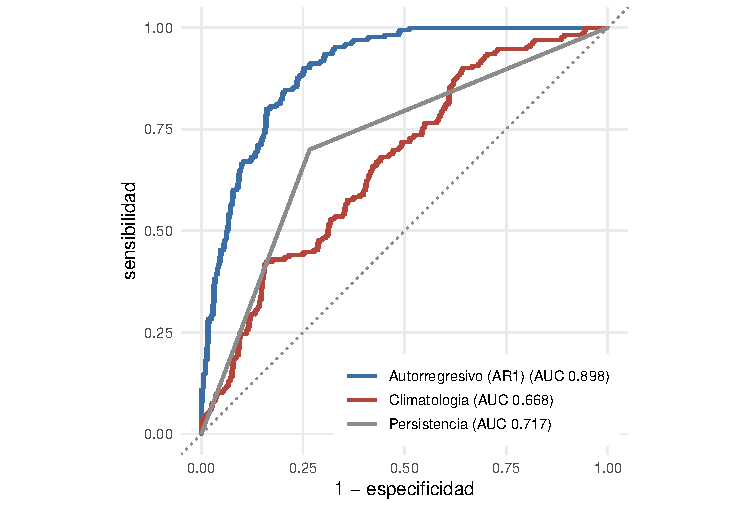
\includegraphics[width=\linewidth]{nowcast_roc.pdf}
  \caption{ROC curves in validation (2025) of the autoregressive model and
    the two baselines. Persistence produces three vertices because its
    predictor is binary.}
  \label{fig:nowcast-roc}
\end{figure}

A high AUC is not enough; it must be compared with what would be obtained
without a model. The two baselines are climatology (calendar only, AUC 0.668)
and persistence (today will be like yesterday, AUC 0.717). The model reaches
0.898 in 2025 and outperforms both with $p<10^{-5}$ in DeLong's test
(\cref{fig:nowcast-roc}). With Youden's threshold set on the fitting data
(0.327), not on the validation data, sensitivity is 0.759 and specificity
0.841: of 170 exceedance days it detects 129, with 31 false alarms in 195
clean days.

Leave-one-year-out cross-validation separates the performance on the
partition from the performance expected in an arbitrary year: the AUC ranges
from 0.840 (2021) to 0.915 (2024), with a pooled value of 0.878, 95\,\% CI
$[0.859, 0.897]$. That second figure is the generalization estimate; the
0.898 of 2025 falls within the range. The year effect is not explained by
prevalence or by station coverage, and it is the main limitation of the
model.

Two caveats bound the reading. The model underpredicts in 2025 (mean
prediction 0.338 versus 0.466 observed) because of the 2024 level step, and
it is not recalibrated because that would fit a parameter to the test
period. And it is \emph{nowcasting}, not forecasting: the factors are from
the same day as the response, so the model distinguishes days within a
season ---which climatology cannot do--- but does not anticipate tomorrow's
ozone.


\section{Results}
\label{sec:resultados}

\Cref{tab:resultados} consolidates the performance of the three classifiers
on the 2025 validation together with the two baselines of the autoregressive
model, and \cref{tab:resultados-ejes} summarizes what each interdependence
technique delivered. The three classifiers exceed the 0.75 performance
threshold set in \cref{sec:obj:objetivo}.

\begin{table}[t]
  \centering
  \caption{Performance on the 2025 validation. The station-day models
    (logistic and discriminant) and the metropolitan-area model
    (autoregressive and its baselines) answer different questions, and their
    AUCs are not directly comparable across blocks. Sensitivity and
    specificity at the Youden threshold set on the fitting data;
    generalization is the out-of-sample AUC from leave-one-year-out
    cross-validation.}
  \label{tab:resultados}
  \small
  \begin{tabular}{lrrrr}
    \toprule
    Model & AUC & Sens. & Spec. & General. \\
    \midrule
    \multicolumn{5}{l}{\emph{Station-day} ($n=2{,}927$)} \\
    Logistic regression    & 0.850 & 0.698 & 0.853 & 0.80 \\
    Linear discriminant    & 0.846 & 0.758 & 0.788 & 0.80 \\
    \midrule
    \multicolumn{5}{l}{\emph{Metropolitan area} ($n=365$)} \\
    Autoregressive AR(1)   & 0.898 & 0.759 & 0.841 & 0.878 \\
    Climatology (baseline) & 0.668 & ---   & ---   & --- \\
    Persistence (baseline) & 0.717 & ---   & ---   & --- \\
    \bottomrule
  \end{tabular}
\end{table}

\begin{table}[t]
  \centering
  \caption{Axes retained by the interdependence techniques on the 2021--2024
    fitting data. Variance: total for PCA, common for FA.}
  \label{tab:resultados-ejes}
  \small
  \begin{tabular}{llr}
    \toprule
    Technique & Axis & Var. (\%) \\
    \midrule
    \multirow{3}{*}{PCA (15 variables)}
      & Primary combustion load      & 26.1 \\
      & Photochemical forcing        & 19.8 \\
      & Atmospheric stagnation       & 10.0 \\
    \midrule
    \multirow{3}{*}{FA (13 variables)}
      & Primary combustion           & 15.7 \\
      & Ventilation                  & 14.5 \\
      & Photochemical forcing        & 10.1 \\
    \bottomrule
  \end{tabular}
\end{table}

Four results cut across the techniques. First, the same three axes emerge
along two different paths, and FA corrects PCA on one point: the stagnation
axis was a wind axis, because barometric pressure has a communality of 0.13
and almost all of its variance is specific. Second, the hierarchy of effects
is stable across the three classifiers: photochemical forcing weighs more
than primary combustion, ventilation protects, and in the station-day models
season and zone weigh more than any factor. Third, temporal dependence is
real and exploitable: the response lag raises the metropolitan-area AUC from
0.882 to 0.898 and multiplies the odds by 3.83. Fourth, all models share a
year effect that no predictor explains: 2024 and 2025 are the highest-ozone
years of the series and also the best classified, and the performance
expected in an arbitrary year is between 0.02 and 0.05 below that of the
validation.


\section{Discussion and conclusions}
\label{sec:conclusiones}

\subsection{Discussion}

The objective was to classify each station-day as an exceedance or not of
the MDA8 at 51 ppb from same-day conditions, with an AUC of at least 0.75,
and to identify the latent conditions that explain that classification. It
is met: the three classifiers exceed the threshold, and the interdependence
techniques produce three axes with a physical interpretation that is stable
outside the fitting period.

Ozone exceedance in the MMA is, above all, a seasonal and regional
phenomenon. Season and zone are the predictors with the largest effects in
the station-day models ---spring triples the odds of winter--- and
photochemical forcing, the axis of temperature, radiation and dryness, is the
dominant continuous factor. That forcing weighs more than the precursor load
is consistent with the chemistry of ozone as a secondary pollutant: the
ingredients are necessary, but it is the available energy that sets the rate
of the reactions. Ventilation is the only protective mechanism measured, and
FA shows that it is wind, not pressure, that defines this axis.

Against that seasonal background there is a spatial signal that the measured
meteorology does not explain. For the same season and conditions, the
Northwest and Southwest almost quadruple the odds of the Northeast, and a
station's exceedance rate correlates at 0.83 with its elevation. The
prevailing easterly wind carries the precursors toward the foot of the
mountains, where the orography blocks their exit; the west--east ordering is
stable across the four seasons. The zone contrasts, however, rest on 15
spatial units, and their precision is what 15 units can provide.

Temporal dependence is the third finding. Day-to-day autocorrelation survives
the seasonal decomposition in the four metropolitan-area series, and a single
lag of the response captures almost all of that dependence: having exceeded
yesterday almost quadruples the odds of exceeding today, controlling for
factors and calendar. The autoregressive model distinguishes days within a
season, which climatology cannot do.

Two limitations bound all of the above. The first is the year effect: 2024
and 2025 have an exceedance level that the factors do not explain, and no
model generalizes as well to 2021 as to 2024. With these data it cannot be
decided whether this is a change in emissions, in instrumentation, or two
meteorologically atypical years. The second is the absence of volatile
organic compounds: without them, the axes are described as consistent with
combustion, ventilation or photochemistry, and no statement about the regime
that limits ozone formation can be answered.

\subsection{Conclusions}

\begin{enumerate}[label=\roman*.]
  \item The three classifiers reach AUCs from 0.846 to 0.898 in 2025 and
    exceed the performance threshold. The logistic model and the
    discriminant are equivalent in practice, so the interpretation of the
    odds ratios does not depend on the normality assumption.
  \item Exceedance is mainly seasonal and regional: season and zone weigh
    more than any continuous factor, and among these photochemical forcing
    (2.78 per standard deviation) dominates primary combustion (1.92);
    ventilation protects (0.90).
  \item There is a spatial signal not explained by the measured meteorology:
    the west of the MMA almost quadruples the odds of the Northeast, in
    correspondence with elevation and the prevailing wind.
  \item The working calendar has little influence; only Sunday has a clear,
    small effect, and the Saturday effect disappears when standard errors
    are corrected for dependence.
  \item Day-to-day dependence is genuine and an AR(1) model exploits it: it
    outperforms climatology and persistence with an expected generalization
    of 0.878.
\end{enumerate}

\subsection{Recommendations}

For air quality management, the autoregressive model on the
metropolitan-area series can operate as an exceedance \emph{nowcasting}
system with same-day measurements, with a decision threshold that favors
sensitivity, because the cost of failing to warn of a bad day exceeds that of
one alert too many. The Northwest and Southwest zones deserve specific
monitoring and control measures, since their risk exceeds what their
meteorological conditions explain. And adding volatile organic compound
measurements to the SIMA network is the only way to move from associations
to mechanism.

For the analysis, three methodological improvements are identified:
estimating the Box-Cox parameter on the fitting data only, to close the only
remaining leak; including a moving-average term on the residuals, justified by
the second-order residual of the autoregressive model; and extending the
model to forecasting by lagging the factors, with its own validation.

\subsection{Open questions}

\begin{itemize}
  \item What produced the 2024 step? Distinguishing between a change in
    emissions, in instrumentation, and atypical years requires emission
    inventories and calibration logs that this work did not have.
  \item What characteristic of the west explains the excess risk that the
    zone retains after controlling for meteorology? Land use, distance to
    industrial sources and orographic recirculation are the candidates.
  \item How much of the season effect is photochemistry and how much is
    wind regime? The factors capture it in part, but season retains an
    effect of its own that suggests an unmeasured seasonal variable.
  \item Up to what horizon is forecasting useful? The 1.3-day mixing time of
    the binary chain suggests that beyond two or three days the prediction
    converges to the monthly climatology.
\end{itemize}


\section*{Code availability and use of artificial intelligence}
\label{sec:disponibilidad-ia}

The consolidation, cleaning, aggregation and modeling code, the notebooks with
all results, and the source of this document are available at
\url{https://github.com/Lunaaaalj/MA2003B.102.07}.

Claude (Anthropic), through Claude Code, was used as an assistant to write and
debug the processing and analysis code and to copyedit the text. The research
question, the choice of techniques, the decision criteria and the
interpretation of the results are the authors' own; every figure reported
comes from running the published code. The authors reviewed the content and
take full responsibility for it.


\printbibliography

\appendix
\section{Discarded techniques and decisions}\label{sec:tecnicas-descartadas}

Besides its final result, the factor analysis (\cref{sec:analisis-factorial})
produced three methodological choices that were tried and explicitly
rejected, and two variables that the model could not accommodate. Documenting
them prevents them from looking like omissions: each was discarded for a
concrete, verifiable reason, not for convenience.

\subsection{Horn's parallel analysis}

This is the standard criterion for deciding how many factors to retain, and
here it retains seven ---more than twice the number given by Velicer's MAP,
which was finally adopted. It is not followed, because the result is an
artifact of sample size rather than a substantive signal: the simulated
threshold lies at 0.06 on the reduced matrix and at 1.06 on the full matrix.
With the 16,028 training observations of the 14-predictor block, the
eigenvalues that pure noise would produce concentrate very tightly around
their expected value, the simulation band narrows almost to a point, and any
barely positive eigenvalue exceeds it. The argument for discarding it holds by
looking at the simulated thresholds alone, without examining a single factor
loading. Velicer's MAP is used instead because it is a descriptive minimum
that does not include $n$ in its formula and does not inflate with sample
size.

\subsection{Maximum likelihood extraction}

The extraction of \cref{sec:analisis-factorial} uses iterated principal axes
rather than maximum likelihood, which requires multivariate normality. The
Box-Cox transformations of \cref{sec:transformaciones} brought the marginals
close to symmetry ($|\text{skewness}|<0.5$) but did not make them normal, so
that assumption does not hold for these data. The principal axis solution was
validated against the reference implementation of the R package
\texttt{psych} on the same block: it matches up to the order and sign of the
factors, with communalities equal to the third decimal.

\subsection{Oblique rotation}

Before adopting varimax, an oblique rotation (oblimin), which allows the
factors to correlate, was tried. It found correlations of up to 0.32 between
them ---physically reasonable, since wind disperses pollutants and is not
independent of the combustion load. It is rejected for the instrumental use of
the scores: the goal of \cref{sec:clasificacion_tecs} is to have
non-collinear predictors, and an oblique solution reintroduces exactly the
multicollinearity problem that factor analysis was meant to solve. The
correlation between factors is reported as a finding but is not carried into
the classification model.

\subsection{Two variables the factor model could not accommodate}

\texttt{NOX} and \texttt{RH\_min\_diurna} produced communalities greater than
1 ---the so-called \textbf{Heywood cases}, impossible because communality is a
proportion of variance. \texttt{NOX} is, by chemical definition, the sum of
\texttt{NO} and \texttt{NO2} ($r=0.985$ against that sum): it is not redundant
in an ordinary statistical sense but an accounting identity that the PCA of
\cref{sec:pca} absorbed without complaint and that factor analysis cannot
split into communality and uniqueness. \texttt{RH\_min\_diurna} correlates at
0.892 with \texttt{RH\_media}; unlike \texttt{NOX} it is not an identity, so
\cref{sec:analisis-factorial} kept it under observation until the second fit,
with the full diagnosis, forced the same exit. Both were removed from the
predictor block, which is left with 13 variables and a maximum VIF of 2.54.
That PCA flagged neither problem is itself a result: the factor model exposes
redundancies that a total-variance decomposition has no way of reporting.

\section{Data dictionary}\label{sec:diccionario}

This appendix documents the consolidated dataset produced by
\texttt{src/importar\_datos.py} from the six annual SIMA workbooks
(\texttt{data/raw/BD 2020.xlsx} to \texttt{data/raw/BD 2025.xlsx}): what each
variable contains, how the stations are covered, and which quality anomalies
must be addressed before any multivariate analysis.

\subsection{Size of the dataset}\label{sec:dic:dimension}

The consolidated dataset has 754\,603 rows and 18 columns: 3 identifiers and
15 measured parameters. Each row is one station in one hour, coverage runs
from 1 January 2020 at 00:00 to 31 December 2025 at 23:00, and there are no
duplicate records. Of the 11\,319\,045 parameter cells, 1\,188\,343 are
empty: 10.50\,\% missing.

At the source, each annual workbook has one sheet per station ---13 in 2020,
14 in 2021 and 15 from 2022 onward--- in wide format: one row per hour and one
column per parameter. There is no station column; consolidation promotes the
sheet name to the \texttt{estacion} column and stacks the six years.

\subsection{Identifier variables}\label{sec:dic:identificadoras}

\begin{description}
  \item[\texttt{fecha}] Timestamp of the observation (date), at hourly
    resolution (\texttt{datetime64}), from 2020-01-01 00:00 to 2025-12-31
    23:00. No missing values.
  \item[\texttt{estacion}] Nominal categorical variable (station) with 15
    levels: CE, NE, NE2, NE3, NO, NO2, NO3, NTE, NTE2, SE, SE2, SE3, SO, SO2
    and SUR. No missing values.
  \item[\texttt{anio}] Calendar year, derived from the source file. Discrete
    numeric (or ordinal categorical), with values from 2020 to 2025. No
    missing values.
\end{description}

\subsection{Criteria pollutants}\label{sec:dic:contaminantes}

The eight criteria pollutants are continuous numeric variables and are
summarized in \cref{tab:dic-contaminantes}. The reported operating range spans
from the most restrictive to the most permissive year of the period, because
the limit changes from year to year (\cref{sec:dic:rangos}). According to
\texttt{Etiquetas.xlsx}, O$_3$, SO$_2$ and NO$_2$ can be converted to ppm by
dividing by 1000.

\subsection{Meteorological parameters}\label{sec:dic:meteorologicos}

The seven meteorological parameters appear in \cref{tab:dic-meteo}. Two of
them cannot be treated as ordinary continuous variables:

\begin{itemize}
  \item \texttt{WDR} is a \textbf{circular} variable, even though it is stored
    as a number: $0^{\circ}$ and $360^{\circ}$ are the same direction (north).
    It cannot be averaged, scaled or correlated like the others; it must be
    decomposed into $\sin\theta$ and $\cos\theta$, or into the wind components
    $u = -\,\mathrm{WSR}\cdot\sin\theta$ and
    $v = -\,\mathrm{WSR}\cdot\cos\theta$. It is a derived attribute that must
    be built at the transformation stage.
  \item \texttt{RAINF} and \texttt{SR} are \textbf{zero-inflated}: 98.4\,\% of
    the valid precipitation records and 39.6\,\% of the solar radiation
    records are exactly zero (night and days without rain). These are
    legitimate zeros, not missing values or errors, but they break normality
    assumptions and distort any standardization.
\end{itemize}

\subsection{Station catalog}\label{sec:dic:estaciones}

\Cref{tab:dic-estaciones} lists the 15 stations with the description from
\texttt{Etiquetas.xlsx} and the coverage computed on the consolidated
dataset. Two stations are not documented in the SIMA catalog and also joined
the network late: NE3 appears from 2021 and NO3 only from December 2022, so
any analysis that requires the full panel must exclude them or be trimmed to
the common period.

\subsection{Quality flags}\label{sec:dic:banderas}

SIMA documents in \texttt{Etiquetas.xlsx} a system of flags that records why
an hour is invalidated (\cref{tab:dic-banderas}). These flags \textbf{are not
included in the \texttt{BD *.xlsx} files}: the delivered workbooks contain
only the numeric value or an empty cell. The data arrive already filtered;
each empty cell is an hour that SIMA invalidated for one of those reasons, but
the reason cannot be recovered.

The methodological consequence is direct: the missing values in this dataset
\textbf{are not random} (not MCAR). They concentrate where there was
calibration, failure or an anomalous condition, which brings them closer to a
MAR mechanism. This constrains which imputation is defensible, and it must be
declared as an assumption.

\subsection{Missing data}\label{sec:dic:faltantes}

\Cref{tab:dic-faltantes} gives the percentage of missing values per variable,
which ranges from 3.66\,\% for \texttt{SR} to 25.23\,\% for \texttt{PM2.5}.
That average hides what matters: missingness is not evenly distributed across
stations or years.

For ozone, \textbf{2020 is practically unusable}
(\cref{tab:dic-o3-faltante}): NTE, SUR and SE2 have 100\,\% of ozone missing
that year, NE 99.9\,\%, NO 98.4\,\%, NTE2 93.3\,\% and NE2 89.1\,\%. From
2022 onward, missing O$_3$ falls to between 1\,\% and 8\,\% across almost the
entire network; the exception is NO3, with 30.3\,\% in 2025.

\subsection{Sentinel and physically impossible values}\label{sec:dic:centinela}

\Cref{tab:dic-anomalias} gathers the values that cannot be taken as
measurements. The clearest case is $-9999$, the missing-data code of the
\emph{datalogger}: 26 cells spread across NOX, RAINF, RH, SR, TOUT, WSR and
WDR are enough to shift means and correlations, so they must be converted to
\texttt{NaN} before any computation.

\subsection{Operating ranges are not stable across years}\label{sec:dic:rangos}

The SIMA range document defines different limits for each year, and some are
stricter than the actual data. The critical case is \texttt{PRS}: the range
declared for 2022 is 700--740 mmHg, and with that criterion 6\,305 records of
that year (about 4.8\,\%) would fall outside it, whereas in 2021, 2023, 2024
and 2025 the same kind of reading is valid because the lower limit drops to
687--690. Applying the document literally would delete legitimate data.

The same happens with \texttt{TOUT}, whose declared minimum is $0^{\circ}$C
in 2020 and 2023 but $-6.5^{\circ}$C in 2021: Monterrey has real frosts, so
the $0^{\circ}$C limit is a data-entry error in the document and not a
physical rule.

The adopted criterion is to use the \textbf{manufacturer range}
(\cref{tab:dic-fabricante}), which is physical and stable, as a hard filter
to remove impossible values, and to treat the annual operating range as a
signal of suspicion to review, not as an automatic deletion rule.

\subsection{Incomplete time grid}\label{sec:dic:rejilla}

No station has a complete hourly series: between 3 (CE) and 16 (SUR)
timestamps are missing relative to the continuous hourly grid of its period.
These are missing hours, not empty rows: the row simply does not exist. For
this reason, any temporal interpolation requires reindexing against a
complete hourly grid first; otherwise the method will assume that two
contiguous observations are one hour apart when they are not.

\begin{table*}[t]
  \centering
  \caption{Criteria pollutants. All are continuous numeric variables. The
    operating range goes from the most restrictive to the most permissive
    year of the period.}
  \label{tab:dic-contaminantes}
  \small
  \begin{tabular}{lllcccc}
    \toprule
    Variable & Description & Unit & Operating range & Observed range & Median & \% missing \\
    \midrule
    \texttt{CO}    & Carbon monoxide                       & ppm             & 0--8 to 0--20       & $0.0$--$37.0$    & 1.17  & 13.31 \\
    \texttt{NO}    & Nitric oxide                          & ppb             & 0--350 to 0--500    & $0.3$--$945.1$   & 5.00  & 16.75 \\
    \texttt{NO2}   & Nitrogen dioxide                      & ppb             & 0--100 to 0--200    & $0.0$--$188.6$   & 11.40 & 17.37 \\
    \texttt{NOX}   & Nitrogen oxides (NO $+$ NO$_2$)       & ppb             & 0--400 to 0--500    & $-9999$--$971.8$ & 17.30 & 16.82 \\
    \texttt{O3}    & \textbf{Ozone}: target variable       & ppb             & 0--153 to 0--185    & $0.5$--$265.0$   & 23.00 & 14.73 \\
    \texttt{PM10}  & Particles $<10\,\mu$m                 & $\mu$g/m$^3$    & 0--800 to 0--999    & $1.0$--$1001.0$  & 49.00 & 4.63  \\
    \texttt{PM2.5} & Particles $<2.5\,\mu$m                & $\mu$g/m$^3$    & 0--205.94 to 0--999 & $0.0$--$999.0$   & 17.00 & 25.23 \\
    \texttt{SO2}   & Sulfur dioxide                        & ppb             & 0--150 to 0--405    & $0.0$--$404.7$   & 3.80  & 15.03 \\
    \bottomrule
  \end{tabular}
\end{table*}

\begin{table*}[t]
  \centering
  \caption{Meteorological parameters. All are continuous numeric variables,
    with the caveats of \texttt{WDR} (circular) and of \texttt{RAINF} and
    \texttt{SR} (zero-inflated).}
  \label{tab:dic-meteo}
  \small
  \begin{tabular}{lllcccc}
    \toprule
    Variable & Description & Unit & Operating range & Observed range & Median & \% missing \\
    \midrule
    \texttt{TOUT}  & Ambient temperature  & $^{\circ}$C        & $-6.5$--45 to 0--45.5 & $-9999$--$785.0$ & 24.02  & 6.95  \\
    \texttt{RH}    & Relative humidity    & \%                 & 0--100                & $-9999$--$725.0$ & 59.00  & 11.38 \\
    \texttt{SR}    & Solar radiation      & kW/m$^2$           & 0--1 to 0--1.26       & $-9999$--$604.0$ & 0.00   & 3.66  \\
    \texttt{RAINF} & Precipitation        & mm/h               & 0--25 to 0--80        & $-9999$--$360.0$ & 0.00   & 4.74  \\
    \texttt{PRS}   & Atmospheric pressure & mmHg               & 687.5--750            & $0.0$--$750.0$   & 714.40 & 5.08  \\
    \texttt{WSR}   & Wind speed           & km/h               & 0--35 to 0--75        & $-9999$--$337.0$ & 7.40   & 6.87  \\
    \texttt{WDR}   & Wind direction       & azimuth degrees    & 0--360                & $-9999$--$360.0$ & 116.00 & 8.35  \\
    \bottomrule
  \end{tabular}
\end{table*}

\begin{table*}[t]
  \centering
  \caption{Catalog of monitoring stations. The description comes from
    \texttt{Etiquetas.xlsx}; coverage and hours were computed on the
    consolidated dataset.}
  \label{tab:dic-estaciones}
  \small
  \begin{tabular}{lllllr}
    \toprule
    Code & Name & Site & Municipality & Coverage & Hours \\
    \midrule
    \texttt{CE}   & Centro                & Obispado       & Monterrey                & 2020--2025                & 52\,605 \\
    \texttt{NE}   & Noreste               & San Nicolás    & San Nicolás de los Garza & 2020--2025                & 52\,595 \\
    \texttt{NE2}  & Noreste 2             & Apodaca        & Apodaca                  & 2020--2025                & 52\,593 \\
    \texttt{NE3}  & \emph{Undocumented}   & ---            & ---                      & \textbf{2021--2025}       & 43\,817 \\
    \texttt{NO}   & Noroeste              & San Bernabé    & Monterrey                & 2020--2025                & 52\,597 \\
    \texttt{NO2}  & Noroeste 2            & García         & García                   & 2020--2025                & 52\,594 \\
    \texttt{NO3}  & \emph{Undocumented}   & ---            & ---                      & \textbf{Dec.\ 2022--2025} & 27\,045 \\
    \texttt{NTE}  & Norte                 & Escobedo       & Escobedo                 & 2020--2025                & 52\,595 \\
    \texttt{NTE2} & Norte 2               & Universidad    & (not given)              & 2020--2025                & 52\,593 \\
    \texttt{SE}   & Sureste               & La Pastora     & Guadalupe                & 2020--2025                & 52\,599 \\
    \texttt{SE2}  & Sureste 2             & Juárez         & Juárez                   & 2020--2025                & 52\,595 \\
    \texttt{SE3}  & Sureste 3             & Cadereyta      & (not given)              & 2020--2025                & 52\,593 \\
    \texttt{SO}   & Suroeste              & Santa Catarina & Santa Catarina           & 2020--2025                & 52\,597 \\
    \texttt{SO2}  & Suroeste 2            & San Pedro      & San Pedro Garza García   & 2020--2025                & 52\,593 \\
    \texttt{SUR}  & Sur                   & Pueblo Serena  & (not given)              & 2020--2025                & 52\,592 \\
    \bottomrule
  \end{tabular}
\end{table*}

\begin{table*}[t]
  \centering
  \caption{Quality flags documented in \texttt{Etiquetas.xlsx}. They do not
    appear in the \texttt{BD *.xlsx} workbooks, so the reason for
    invalidation cannot be recovered from the delivered data.}
  \label{tab:dic-banderas}
  \small
  \begin{tabular}{llcc}
    \toprule
    Flag & Cause & Valid-hour mark & Invalid-hour mark \\
    \midrule
    \texttt{P} / \texttt{p} & Power failure                                      & \texttt{P} & \texttt{p} \\
    \texttt{C} / \texttt{c} & Calibration                                        & \texttt{C} & \texttt{c} \\
    \texttt{D} / \texttt{d} & Shutdown                                           & \texttt{D} & \texttt{d} \\
    \texttt{B} / \texttt{b} & Bad conditions                                     & \texttt{B} & \texttt{b} \\
    \texttt{m}              & Positive above range                               & ---        & \texttt{m} \\
    \texttt{l}              & Negative below range or solar radiation adjustment & ---        & \texttt{l} \\
    \texttt{z}              & Zeros and negatives                                & ---        & \texttt{z} \\
    \texttt{o}              & PM10 above $900\,\mu$g/m$^3$                       & ---        & \texttt{o} \\
    \texttt{s}              & Repeated or identical consecutive values           & ---        & \texttt{s} \\
    \texttt{r}              & PM10 versus PM2.5 comparison                       & ---        & \texttt{r} \\
    \texttt{e}              & Delete NO and NOx data                             & ---        & \texttt{e} \\
    \texttt{a}              & Delete PM $<5\,\mu$g/m$^3$ and CO $<0.05$ ppm      & ---        & \texttt{a} \\
    \texttt{f}              & Value $3\times$ the previous one (PM10)            & ---        & \texttt{f} \\
    \texttt{h}              & Jump $>10^{\circ}$C or $>10$ mmHg from the previous hour & --- & \texttt{h} \\
    \texttt{n}              & Communication failure                              & ---        & \texttt{n} \\
    \texttt{x}              & Value that passed the protocols but should not be present & --- & \texttt{x} \\
    \texttt{u}              & Undocumented                                       & \multicolumn{2}{c}{Undocumented} \\
    \bottomrule
  \end{tabular}
\end{table*}

\begin{table}[t]
  \centering
  \caption{Percentage of missing values per variable.}
  \label{tab:dic-faltantes}
  \small
  \begin{tabular}{lr@{\qquad}lr}
    \toprule
    Variable & \% missing & Variable & \% missing \\
    \midrule
    \texttt{PM2.5} & 25.23 & \texttt{RH}    & 11.38 \\
    \texttt{NO2}   & 17.37 & \texttt{WDR}   & 8.35  \\
    \texttt{NOX}   & 16.82 & \texttt{TOUT}  & 6.95  \\
    \texttt{NO}    & 16.75 & \texttt{WSR}   & 6.87  \\
    \texttt{SO2}   & 15.03 & \texttt{PRS}   & 5.08  \\
    \texttt{O3}    & 14.73 & \texttt{RAINF} & 4.74  \\
    \texttt{CO}    & 13.31 & \texttt{PM10}  & 4.63  \\
                   &       & \texttt{SR}    & 3.66  \\
    \bottomrule
  \end{tabular}
\end{table}

\begin{table}[t]
  \centering
  \caption{Percentage of missing O$_3$ by station and year. A dash indicates
    that the station was not yet operating.}
  \label{tab:dic-o3-faltante}
  \small
  \begin{tabular}{lrrrrrr}
    \toprule
    Station & 2020 & 2021 & 2022 & 2023 & 2024 & 2025 \\
    \midrule
    \texttt{CE}   & 16.5  & 12.2 & 3.6 & 4.1  & 4.2  & 3.4  \\
    \texttt{NE}   & 99.9  & 16.0 & 3.8 & 5.0  & 3.7  & 10.1 \\
    \texttt{NE2}  & 89.1  & 18.6 & 3.3 & 7.8  & 7.0  & 6.0  \\
    \texttt{NE3}  & ---   & 4.9  & 4.4 & 4.2  & 5.2  & 7.6  \\
    \texttt{NO}   & 98.4  & 20.3 & 6.2 & 6.0  & 11.0 & 7.4  \\
    \texttt{NO2}  & 20.3  & 5.9  & 2.4 & 2.7  & 3.8  & 4.7  \\
    \texttt{NO3}  & ---   & ---  & 5.1 & 16.5 & 3.5  & 30.3 \\
    \texttt{NTE}  & 100.0 & 18.5 & 4.3 & 7.3  & 4.0  & 4.2  \\
    \texttt{NTE2} & 93.3  & 9.5  & 2.5 & 2.9  & 5.9  & 4.6  \\
    \texttt{SE}   & 7.3   & 5.6  & 2.7 & 2.8  & 2.8  & 3.0  \\
    \texttt{SE2}  & 100.0 & 39.3 & 5.5 & 1.6  & 12.0 & 10.0 \\
    \texttt{SE3}  & 28.5  & 5.9  & 1.8 & 4.7  & 1.4  & 0.5  \\
    \texttt{SO}   & 31.0  & 7.0  & 5.4 & 4.3  & 5.9  & 4.7  \\
    \texttt{SO2}  & 3.0   & 2.5  & 2.6 & 1.9  & 1.4  & 1.4  \\
    \texttt{SUR}  & 100.0 & 16.4 & 2.6 & 2.8  & 0.9  & 0.9  \\
    \bottomrule
  \end{tabular}
\end{table}

\begin{table*}[t]
  \centering
  \caption{Sentinel and physically impossible values detected in the
    consolidated dataset.}
  \label{tab:dic-anomalias}
  \small
  \begin{tabular}{p{3cm}p{2.6cm}rp{7cm}}
    \toprule
    Anomaly & Affected variables & $n$ & Interpretation \\
    \midrule
    $-9999$
      & NOX, RAINF, RH, SR, TOUT, WSR, WDR & 26
      & Missing-data code of the \emph{datalogger}, \textbf{not a value}. Must be set to \texttt{NaN} before any computation. \\
    \addlinespace
    $\mathrm{RH} > 100$\,\% & RH & 285
      & Impossible by definition; maxima of 714\,\% and 725\,\% are observed. \\
    \addlinespace
    $\mathrm{TOUT} > 50^{\circ}$C & TOUT & 3
      & Outside the sensor range ($-50$ to $50^{\circ}$C); the observed maximum is $785^{\circ}$C. \\
    \addlinespace
    \texttt{SR} on the wrong scale & SR & $\approx 30$
      & Values of 64, 501 and 604 against a physical maximum of 1.4 kW/m$^2$: readings in W/m$^2$ mixed in (divide by 1000). \\
    \addlinespace
    \texttt{SR} between 1.5 and 7.8 & SR & $\approx 730$
      & Exceed the manufacturer range and concentrate at NTE (493) and SO (172), which suggests sensor failure or miscalibration rather than a meteorological event. \\
    \addlinespace
    $\mathrm{WSR} > 100$ km/h & WSR & 418
      & Above any wind recorded in the MMA; 306 of them occur in 2021. \\
    \addlinespace
    $\mathrm{PRS} = 0$ or $\mathrm{PRS} < 500$ & PRS & 2
      & A zero atmospheric pressure is impossible. \\
    \addlinespace
    $\mathrm{PM10} \geq 999$, $\mathrm{PM2.5} = 999$ & PM10, PM2.5 & 6
      & Cap values (999, 1000, 1001) characteristic of saturation or sentinel codes, not real concentrations. \\
    \addlinespace
    $\mathrm{CO} > 18$ ppm & CO & 24
      & Exceeds the operating range of every year; the maximum is 37 ppm. \\
    \bottomrule
  \end{tabular}
\end{table*}

\begin{table}[t]
  \centering
  \caption{Manufacturer range per parameter, adopted as a hard filter for
    impossible values.}
  \label{tab:dic-fabricante}
  \small
  \begin{tabular}{lc}
    \toprule
    Parameter & Manufacturer range \\
    \midrule
    PM10, PM2.5, O3      & $0$--$1000$     \\
    NO, NO2, NOx, SO2    & $0$--$500$      \\
    CO                   & $0$--$50$       \\
    RH                   & $0$--$100$      \\
    WS (\texttt{WSR})    & $0$--$180$      \\
    TEMP (\texttt{TOUT}) & $-50$--$50$     \\
    SR                   & $0$--$1.4$      \\
    BP (\texttt{PRS})    & $449.9$--$824.9$\\
    WD (\texttt{WDR})    & $0$--$360$      \\
    \bottomrule
  \end{tabular}
\end{table}

\section{Dictionary of the transformed data}\label{sec:diccionario-transformado}
This appendix documents the daily dataset that results from the
transformations of \cref{sec:transformaciones}. The file
\texttt{data/processed/sima\_transformado\_diario.parquet} is the input of the
subsequent multivariate analyses.

\subsection{Size and coverage}
The transformed dataset contains 26,691 station-day observations and 34
columns. It comprises 15 stations and covers 1 January 2021 to 31 December
2025. Sixteen measured continuous predictors were transformed and
standardized; the remaining 18 columns were kept on their original scale.

The criterion of \cref{sec:transformaciones} was reapplied to the daily table
without changing the method. Of the 16 continuous variables, 13 required
Box-Cox and $z$-standardization. \texttt{PRS\_media}, \texttt{RH\_media} and
\texttt{RH\_min\_diurna} met the skewness criterion on their original scale
and were only standardized. Missing values were kept without imputation.

\subsection{Variables of the daily dataset}
\Cref{tab:dic-diario-continuas} presents the 16 continuous predictors. Units
refer to the original scale, before transformation and standardization.

\begin{table*}[pos=t]
  \centering
  \caption{Transformed and standardized continuous predictors of the daily
    dataset. Units refer to the original scale.}
  \label{tab:dic-diario-continuas}
  \footnotesize
  \setlength{\tabcolsep}{4pt}
  \begin{tabular}{lp{7.2cm}llr}
    \toprule
    Variable & Description & Unit & Treatment & Missing \\
    \midrule
    \texttt{TOUT\_max} & Daily maximum ambient temperature
      & $^{\circ}\mathrm{C}$ & Box-Cox + z & 1,561 \\
    \texttt{SR\_acum} & Daily total solar radiation
      & $\mathrm{kWh}/\mathrm{m}^{2}$ & Box-Cox + z & 1,123 \\
    \texttt{NO\_06\_09} & Mean NO between 06:00 and 09:00 h
      & ppb & Box-Cox + z & 1,757 \\
    \texttt{NO2\_06\_09} & Mean NO$_2$ between 06:00 and 09:00 h
      & ppb & Box-Cox + z & 1,776 \\
    \texttt{NOX\_06\_09} & Mean NO$_x$ between 06:00 and 09:00 h
      & ppb & Box-Cox + z & 1,790 \\
    \texttt{CO\_06\_09} & Mean CO between 06:00 and 09:00 h
      & ppm & Box-Cox + z & 1,937 \\
    \texttt{WSR\_media} & Daily mean wind speed
      & km/h & Box-Cox + z & 1,008 \\
    \texttt{WSR\_min} & Daily minimum wind speed
      & km/h & Box-Cox + z & 1,008 \\
    \texttt{PRS\_media} & Daily mean atmospheric pressure
      & mmHg & z only & 886 \\
    \texttt{RH\_media} & Daily mean relative humidity
      & \% & z only & 2,649 \\
    \texttt{RH\_min\_diurna} & Daytime minimum relative humidity
      & \% & z only & 2,575 \\
    \texttt{viento\_u\_media} & Daily vector mean of the east--west wind
      component & --- & Box-Cox + z & 1,447 \\
    \texttt{viento\_v\_media} & Daily vector mean of the north--south wind
      component & --- & Box-Cox + z & 1,447 \\
    \texttt{PM10\_media} & Daily mean PM$_{10}$
      & $\mu\mathrm{g}/\mathrm{m}^{3}$ & Box-Cox + z & 940 \\
    \texttt{PM2.5\_media} & Daily mean PM$_{2.5}$
      & $\mu\mathrm{g}/\mathrm{m}^{3}$ & Box-Cox + z & 5,965 \\
    \texttt{SO2\_media} & Daily mean SO$_2$
      & ppb & Box-Cox + z & 1,933 \\
    \bottomrule
  \end{tabular}
\end{table*}

With 2025 complete, the skewness of \texttt{SR\_acum} rises to 0.53 and no
longer meets the criterion, so it is transformed ($\lambda=0.755$); it is
kept as a continuous predictor and is not converted to a binary one. All 16
variables of \cref{tab:dic-diario-continuas} fall within the
$|\mathrm{skewness}|<0.5$ criterion.

\Cref{tab:dic-diario-originales} gathers the 18 columns that were not
transformed. \texttt{msnm} (elevation) is kept because it is an attribute of
the station, with 15 repeated values, not a daily measurement. \texttt{MDA8}
and \texttt{O3\_max\_1h} remain in ppb because they define the target
variables, and their thresholds must keep a direct physical interpretation.

\begin{table*}[pos=t]
  \centering
  \caption{Columns kept on the original scale in the transformed daily
    dataset.}
  \label{tab:dic-diario-originales}
  \footnotesize
  \setlength{\tabcolsep}{4pt}
  \begin{tabular}{llp{8.0cm}lr}
    \toprule
    Variable & Type & Description & Unit & Missing \\
    \midrule
    \texttt{estacion} & nominal & SIMA monitoring station, with 15 levels
      & --- & 0 \\
    \texttt{fecha} & date & Calendar day of the observation
      & --- & 0 \\
    \texttt{zona} & nominal & Geographic zone from the SIMA catalog, with seven
      levels & --- & 0 \\
    \texttt{msnm} & continuous & Station elevation above sea level
      & m & 0 \\
    \texttt{anio} & discrete & Calendar year
      & --- & 0 \\
    \texttt{mes} & discrete & Calendar month
      & --- & 0 \\
    \texttt{temporada} & nominal & Season of the year, with four levels
      & --- & 0 \\
    \texttt{tipo\_dia} & nominal & Weekday, Saturday, Sunday or holiday
      & --- & 0 \\
    \texttt{festivo} & binary & Public holiday indicator
      & 0/1 & 0 \\
    \texttt{fin\_de\_semana} & binary & Saturday or Sunday indicator
      & 0/1 & 0 \\
    \texttt{llovio} & binary & Indicator of at least one hour of the day with
      precipitation & 0/1 & 800 \\
    \texttt{MDA8} & continuous & Daily maximum of the 8-h moving average of
      O$_3$ & ppb & 1,591 \\
    \texttt{ventanas\_validas} & discrete & Number of valid 8-h moving windows
      during the day, out of a maximum of 24 & windows & 0 \\
    \texttt{O3\_max\_1h} & continuous & Hourly maximum of O$_3$ during the day
      & ppb & 838 \\
    \texttt{excede\_anio\_1} & binary & MDA8 exceedance above 65 ppb
      & 0/1 & 1,591 \\
    \texttt{excede\_anio\_3} & binary & MDA8 exceedance above 60 ppb
      & 0/1 & 1,591 \\
    \texttt{excede\_anio\_5} & binary & MDA8 exceedance above 51 ppb
      & 0/1 & 1,591 \\
    \texttt{excede\_1h} & binary & Exceedance of the hourly maximum above
      90 ppb & 0/1 & 0 \\
    \bottomrule
  \end{tabular}
\end{table*}

\subsection{Skewness and kurtosis}
\Cref{tab:dic-diario-sesgo} compares the shape of the distributions before
and after treatment. $z$-standardization is a linear transformation and does
not change skewness or kurtosis. Therefore, the three variables that were only
standardized keep the values of the original scale.

\begin{table*}[pos=t]
  \centering
  \caption{Skewness and excess kurtosis (normal reference equal to zero) of
    the continuous variables of the daily dataset before and after
    treatment.}
  \label{tab:dic-diario-sesgo}
  \small
  \setlength{\tabcolsep}{6pt}
  \begin{tabular}{lrrrrrr}
    \toprule
    & & & \multicolumn{2}{c}{Skewness} & \multicolumn{2}{c}{Kurtosis} \\
    \cmidrule(lr){4-5}\cmidrule(lr){6-7}
    Variable & Shift & $\lambda$ & Before & After & Before & After \\
    \midrule
    \texttt{TOUT\_max} & 1.55 & 2.118 & $-0.86$ & $-0.16$ & 0.60 & $-0.49$ \\
    \texttt{SR\_acum} & 1.00 & 0.755 & 0.53 & 0.00 & 3.04 & 0.99 \\
    \texttt{NO\_06\_09} & 0.00 & $-0.103$ & 4.13 & 0.01 & 32.49 & $-0.09$ \\
    \texttt{NO2\_06\_09} & 1.00 & 0.279 & 1.67 & 0.02 & 6.89 & 0.40 \\
    \texttt{NOX\_06\_09} & 0.00 & 0.008 & 3.04 & 0.00 & 17.68 & 0.52 \\
    \texttt{CO\_06\_09} & 1.00 & $-0.320$ & 1.42 & 0.02 & 4.82 & $-0.53$ \\
    \texttt{WSR\_media} & 0.00 & 0.134 & 8.29 & 0.07 & 149.74 & 3.94 \\
    \texttt{WSR\_min} & 0.00 & 0.285 & 8.74 & 0.04 & 347.89 & 0.94 \\
    \texttt{PRS\_media} & --- & --- & 0.12 & 0.12 & $-0.16$ & $-0.16$ \\
    \texttt{RH\_media} & --- & --- & $-0.37$ & $-0.37$ & 0.19 & 0.19 \\
    \texttt{RH\_min\_diurna} & --- & --- & 0.45 & 0.45 & 0.15 & 0.15 \\
    \texttt{viento\_u\_media} & 116.16 & 2.955 & $-1.74$ & 0.29 & 27.19 & 5.23 \\
    \texttt{viento\_v\_media} & 99.96 & 2.956 & $-1.52$ & 0.20 & 27.68 & 4.86 \\
    \texttt{PM10\_media} & 0.00 & 0.165 & 1.58 & 0.01 & 4.98 & 0.48 \\
    \texttt{PM2.5\_media} & 0.00 & 0.021 & 2.04 & 0.00 & 9.86 & 0.03 \\
    \texttt{SO2\_media} & 0.00 & $-0.202$ & 3.63 & $-0.01$ & 36.70 & 0.47 \\
    \bottomrule
  \end{tabular}
\end{table*}

Daily aggregation reduced the excess kurtosis of the
\texttt{viento\_u\_media} and \texttt{viento\_v\_media} components from 40.5
to 27.2 and from 40.1 to 27.7, respectively. This reduction is about one
third and does not by itself remove the heavy tails. Box-Cox reduces them to
5.23 and 4.86.

The largest kurtosis values before transformation belong to
\texttt{WSR\_min}, with 347.89, and \texttt{WSR\_media}, with 149.74. After
Box-Cox they fall to 0.94 and 3.94. Although all variables meet the skewness
criterion, the residual kurtosis of the wind block should be kept in mind
when interpreting the linear discriminant analysis.



\end{document}
